% This program can be redistributed and/or modified under the terms
% of the GNU Public License, version 3.
%
% Seth Brown, Ph.D.
% sethbrown@drbunsen.org
%
% Compiled with XeLaTeX
% Dependencies:
%   Fontin Sans font (http://www.exljbris.com/fontinsans.html)
%
\documentclass{beamer}

\usepackage{graphicx} % graphics
\usepackage{epsfig} % eps graphics
\usepackage{hyperref} % urls
\usepackage{booktabs, caption} % table styling
\usepackage{subfig}
\usepackage{colortbl}
\usepackage[square,authoryear]{natbib}
\usepackage{pgfpages}
%\setbeameroption{show notes on second screen}
\definecolor{myblue}{HTML}{D4DEFF}
\definecolor{redcell}{HTML}{FFE8E8}
\definecolor{greencell}{HTML}{E8FFEB}
\definecolor{yellowcell}{HTML}{FFFDE8}
\newcommand{\vomega}{\vec{\omega}}
\newcommand{\x}{\mathbf{x}}
\newcommand{\cs}{C_{\phi}(\eta)}
\newcommand{\csinv}{C_{\phi}(1/\eta)}
\newcommand{\ce}{C_{\mathbf{E}}(\eta)}
\newcommand{\gl}[1]{\texttt{\nolinkurl{#1}}}
\newcommand\mycolor[1]{
\ifnum#1>100 \cellcolor{redcell}#1%
\else
\ifnum#1>60 \cellcolor{yellowcell}#1%
\else
\cellcolor{greencell}#1%
\fi
\fi
}% suppress navigation bar
\beamertemplatenavigationsymbolsempty

\mode<presentation>
{
  \usetheme{bunsen}
  \setbeamercovered{transparent}
  \setbeamertemplate{items}[circle]
}

% set fonts
\usepackage{fontspec}
\setsansfont{Fontin Regular}
\setbeamerfont{frametitle}{size=\LARGE,series=\bfseries}

% color definitions
\usepackage{color}
\definecolor{uipoppy}{RGB}{153, 0, 0}
\definecolor{uipaleblue}{RGB}{153,153,153}
\definecolor{uiblack}{RGB}{0, 0, 0}

% caption styling
\DeclareCaptionFont{uiblack}{\color{uiblack}}
\DeclareCaptionFont{uipoppy}{\color{uipoppy}}
\captionsetup{labelfont={uipoppy},textfont=uiblack}

% see the macros.tex file for definitions
% This program can be redistributed and/or modified under the terms
% of the GNU Public License, version 3.

% adds reference to bottom right of corner of a slide
\usepackage[absolute,overlay]{textpos} % text references in slide corners
\newcommand\textref[1]{%
  \begin{textblock*}{\paperwidth}(0pt,0.99\textheight)
  \raggedleft \tiny{\emph{#1}}\hspace{.5em}
  \end{textblock*}}

% for drawing circles around numbers
% ex. \circled{1} Add some text here.
\usepackage{tikz}
\newcommand*\circled[1]{\tikz[baseline=(char.base)]{
            \node[shape=circle,draw,inner sep=2pt] (char) {#1};}}


% title slide definition
\title[Real-time Rendering of Translucent Materials]{Real-time Rendering of Translucent Materials with Directional Subsurface Scattering}
\author{Alessandro Dal Corso}
\institute[DTU Compute]
{
M.Sc. in Digital Media Engineering \\
T.I.M.E. Double Degree Program\\*[2em] 
Supervisor: Jeppe Revall Frisvad
}

\date{22${}^{nd}$ August 2014}

%--------------------------------------------------------------------
%                           Introduction
%--------------------------------------------------------------------

\begin{document}

\section{Introduction}
\setbeamertemplate{background}
{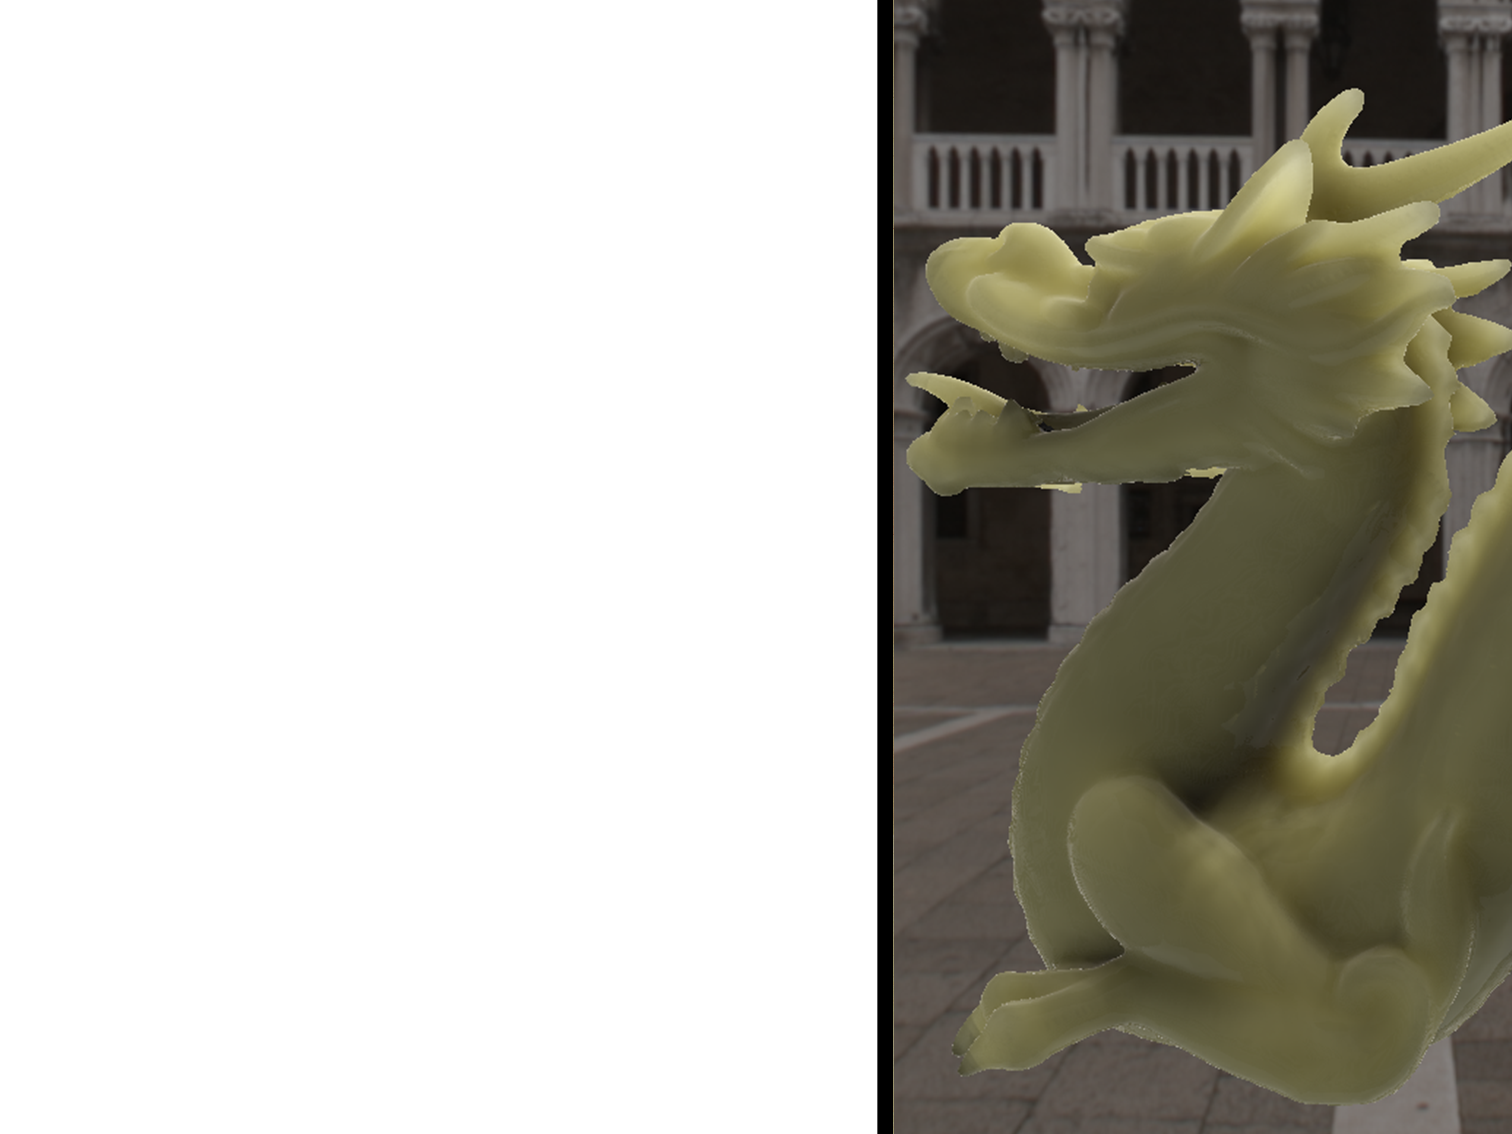
\includegraphics[width=\paperwidth,height=\paperheight]{frontpage_bg}}
\setbeamertemplate{footline}[default]

\begin{frame}
\vspace{1cm}
\begin{columns}
\column{2.75in}
  \titlepage
  \vspace{10cm}
\column{2.0in}
\end{columns}
\note{
\begin{itemize}
\item Alessandro, Msc in DME
\item Thesis title: RTR Translucent Materials with Dir SS
\item DTU Compute
\item Supervisor
\end{itemize}
}
\end{frame}

%-------------------------------------------------------------------
%                          Section 1
%-------------------------------------------------------------------
%
% Set the background for the rest of the slides.
% Insert infoline

\setbeamertemplate{background}
 {
\includegraphics[width=\paperwidth,height=\paperheight]{slide_bg}}
\setbeamertemplate{footline}[bunsentheme]

\section{Introduction}
\begin{frame}
    \frametitle{Introduction}
\begin{columns}[t]
    \begin{column}{0.95\textwidth}
      \centering
			\begin{itemize}
				\item \emph{Subsurface scattering} (SS) is a physical phenomenon that occurs in a wide range of materials (marble, skin, fruit) 
				\item Light repeatedly bounces inside the material and then comes out into another point 
		\vspace{-0.3cm}
		\begin{figure}
		\centering
		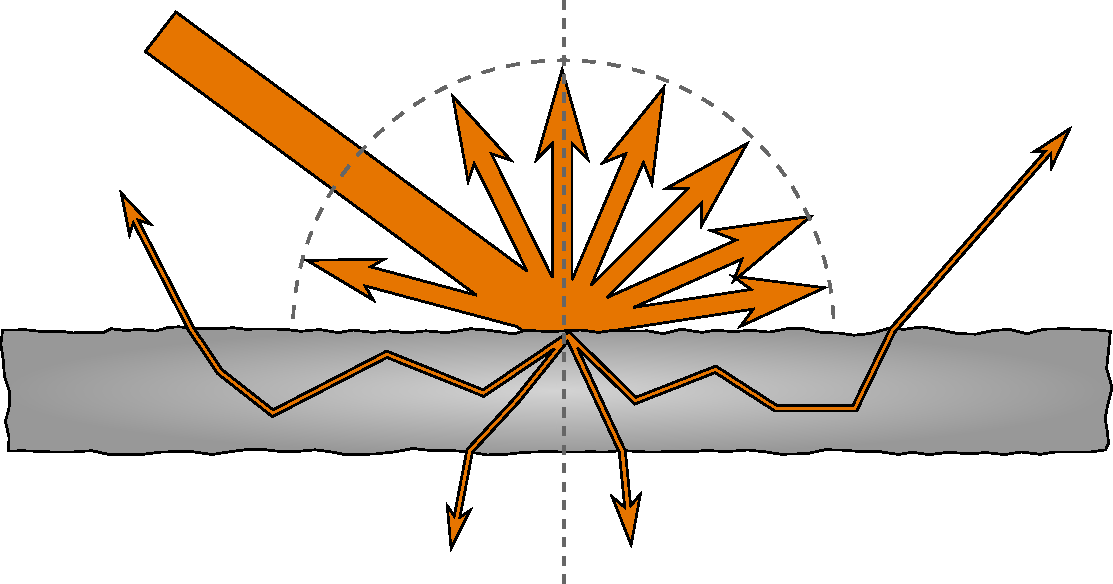
\includegraphics[width=0.7\paperwidth]{diagram}	
		\end{figure}
		\vspace{-0.4cm}
				\item We want to model faithfully SS in a synthetic image
			\end{itemize}
    \end{column}
  \end{columns}
\note{
\begin{itemize}
\item Subsurface scattering: describe in words
\item Light bouncing + comes out (show picture)
\item State problem: physically render faithfully synthetic image
\end{itemize}
}
\end{frame}

\begin{frame}
    \frametitle{Introduction}
\begin{columns}[t]
    \begin{column}{\paperwidth}
      \centering
		\vspace{0.0cm}
		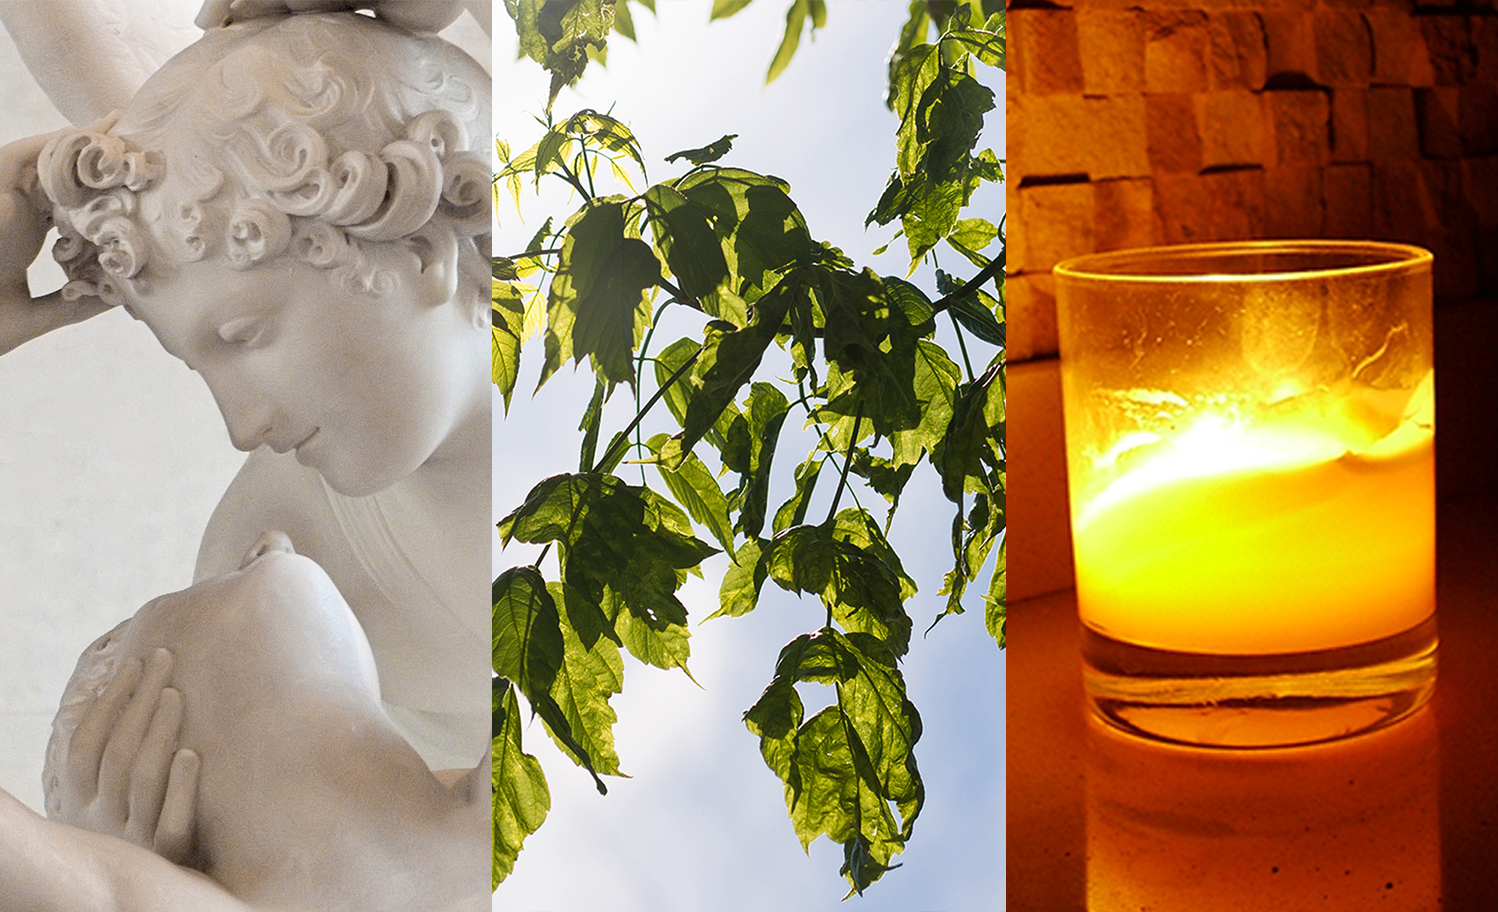
\includegraphics[width=\paperwidth]{comb}
\end{column}
​\end{columns}
\note{
\begin{itemize}
\item Examples in nature
\item Marble, leaves, wax
\item Very present in nature
\end{itemize}
}
\end{frame}

\begin{frame}
    \frametitle{Problem statement}
		Our goal is to faithfully represent SS phenomena in a synthetically generated image:
		\vspace{0.5cm}
		\begin{itemize}
			\item Using a analytical BSSRDF model \citep{IMM2013-06646}  
			\item Visually close as possible to a offline-rendered solution
			\item With low memory requirements 
			\item In real-time or at least at interactive frame rates \\(<100ms per frame) using a GPU-based solution
		\end{itemize}
		\note{
\begin{itemize}
\item Approach
\item Proposal: use an analytical model (BSSRDF) - opposed to numerical
\item Close to offline - never implemented
\item Low memory requirements (console) 
\item Real time - 100 ms - GPUs
\end{itemize}
}
\end{frame}


\section{Theory}
\begin{frame}
    \frametitle{Light transport}
				\vspace{0.5cm}

\begin{columns}
    \begin{column}{0.5\textwidth}
			\begin{itemize}
				\item We define a quantity to describe light carried by a ray, the \emph{radiance}:
			  $$L(\vomega) = \frac{d^2 \Phi}{d\omega dA \cos \theta}$$
			\end{itemize}
    \end{column}
    \begin{column}{0.5\textwidth}
		\centering
		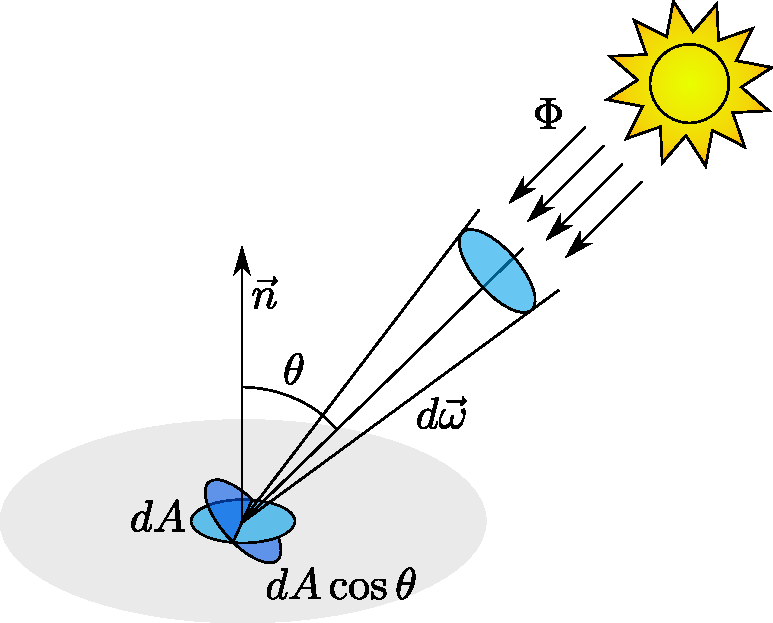
\includegraphics[width=0.7\textwidth]{radiance}
    \end{column}
​  \end{columns}
\vspace{0.3cm}
\begin{columns}
    \begin{column}{0.4\textwidth}
      \centering
		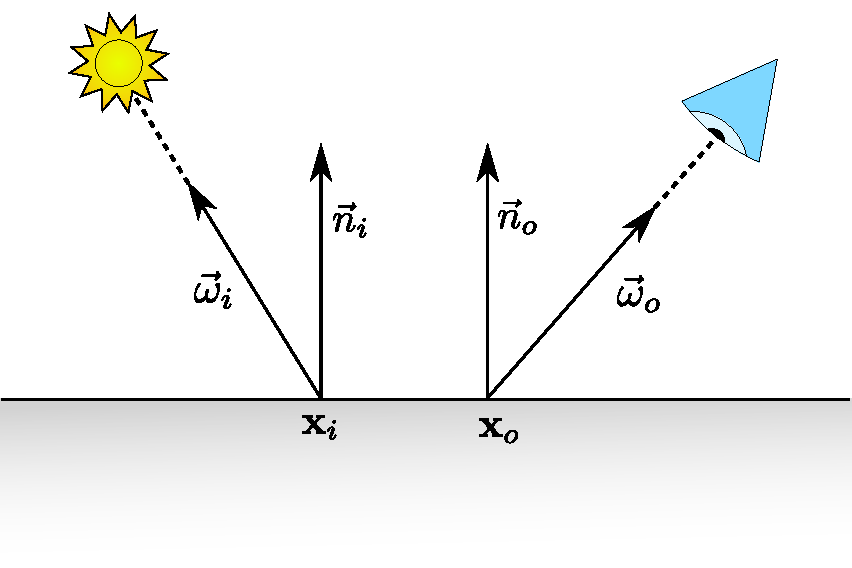
\includegraphics[width=\textwidth]{bssrdf}
				\end{column}
    \begin{column}{0.6\textwidth}
		\begin{itemize}
				\item Given two points on a surface, we define the BSSRDF as:
$$
S(\x_i, \vomega_i, \x_o, \vomega_o) = \frac{d L_o(\x_o,\vomega_o)}{L_i(\x_i,\vomega_i) \cos \theta_i d\vomega_i d A_i}  
$$			
				That relates the entering flux with the exiting radiance.
		\end{itemize}
    \end{column}
​  \end{columns}
\note{
\begin{itemize}
\item small theoretical introduction
\item define radiance and BSSRDF
\item radiance flux over solid angle over projected area
\item radiance and ray
\item 
\end{itemize}
}
\end{frame}

\begin{frame}
    \frametitle{The rendering equation}
			\begin{itemize}
				\item From the definition of BSSRDF we obtain the \emph{area formulation} of the \emph{rendering equation} \citep{Jensen:2001:PMS:383259.383319}:
				$$L_o(\x_o,\vomega_o) = L_e(\x_o,\vomega_o) + \int_A \int_{2\pi} S(\x_i, \vomega_i, \x_o, \vomega_o) L_i(\x_i,\vomega_i) (\vec{n} \cdot \vomega_i) d\vomega_i d A_i$$
				\item Many BSSRDF functions have been proposed in literature \citep{Jensen:2001:PMS:383259.383319,D'Eon:2011:QMR:1964921.1964951,IMM2013-06646}  
			\end{itemize}

\end{frame}

\begin{frame}
    \frametitle{Standard dipole}
			\begin{itemize}
				\item The standard dipole \citep{Jensen:2001:PMS:383259.383319} was one of the first BSSRDF functions proposed
				\item It uses the diffusion approximation \citep{books/daglib/0093591} of the radiative transport equation (RTE)
				\item The approximation describes how light propagates from a point source in an infinite scattering medium:
			\end{itemize}
\begin{equation*}
\phi(\x) = \frac{\Phi}{4\pi D} \frac{e^{\sigma_{tr} r}}{r}
\label{eq:dasimple}
\end{equation*}
$\ \ $Where
$$\phi(\x) = \int_{4\pi}L(\x,\vomega) d\vomega$$
\end{frame}
\begin{frame}
    \frametitle{Standard dipole}
			\begin{itemize}
			\vspace{0.5cm}
				\item For a BSSRDF, we need to put a boundary condition: fluence decreases linearly until a distance $z = 2AD$ from the surface
				\item We model the interaction as two small light point sources, a \textcolor{green}{virtual} and a \textcolor{blue}{real} source \\
				\centering
				\vspace{0.2cm}
				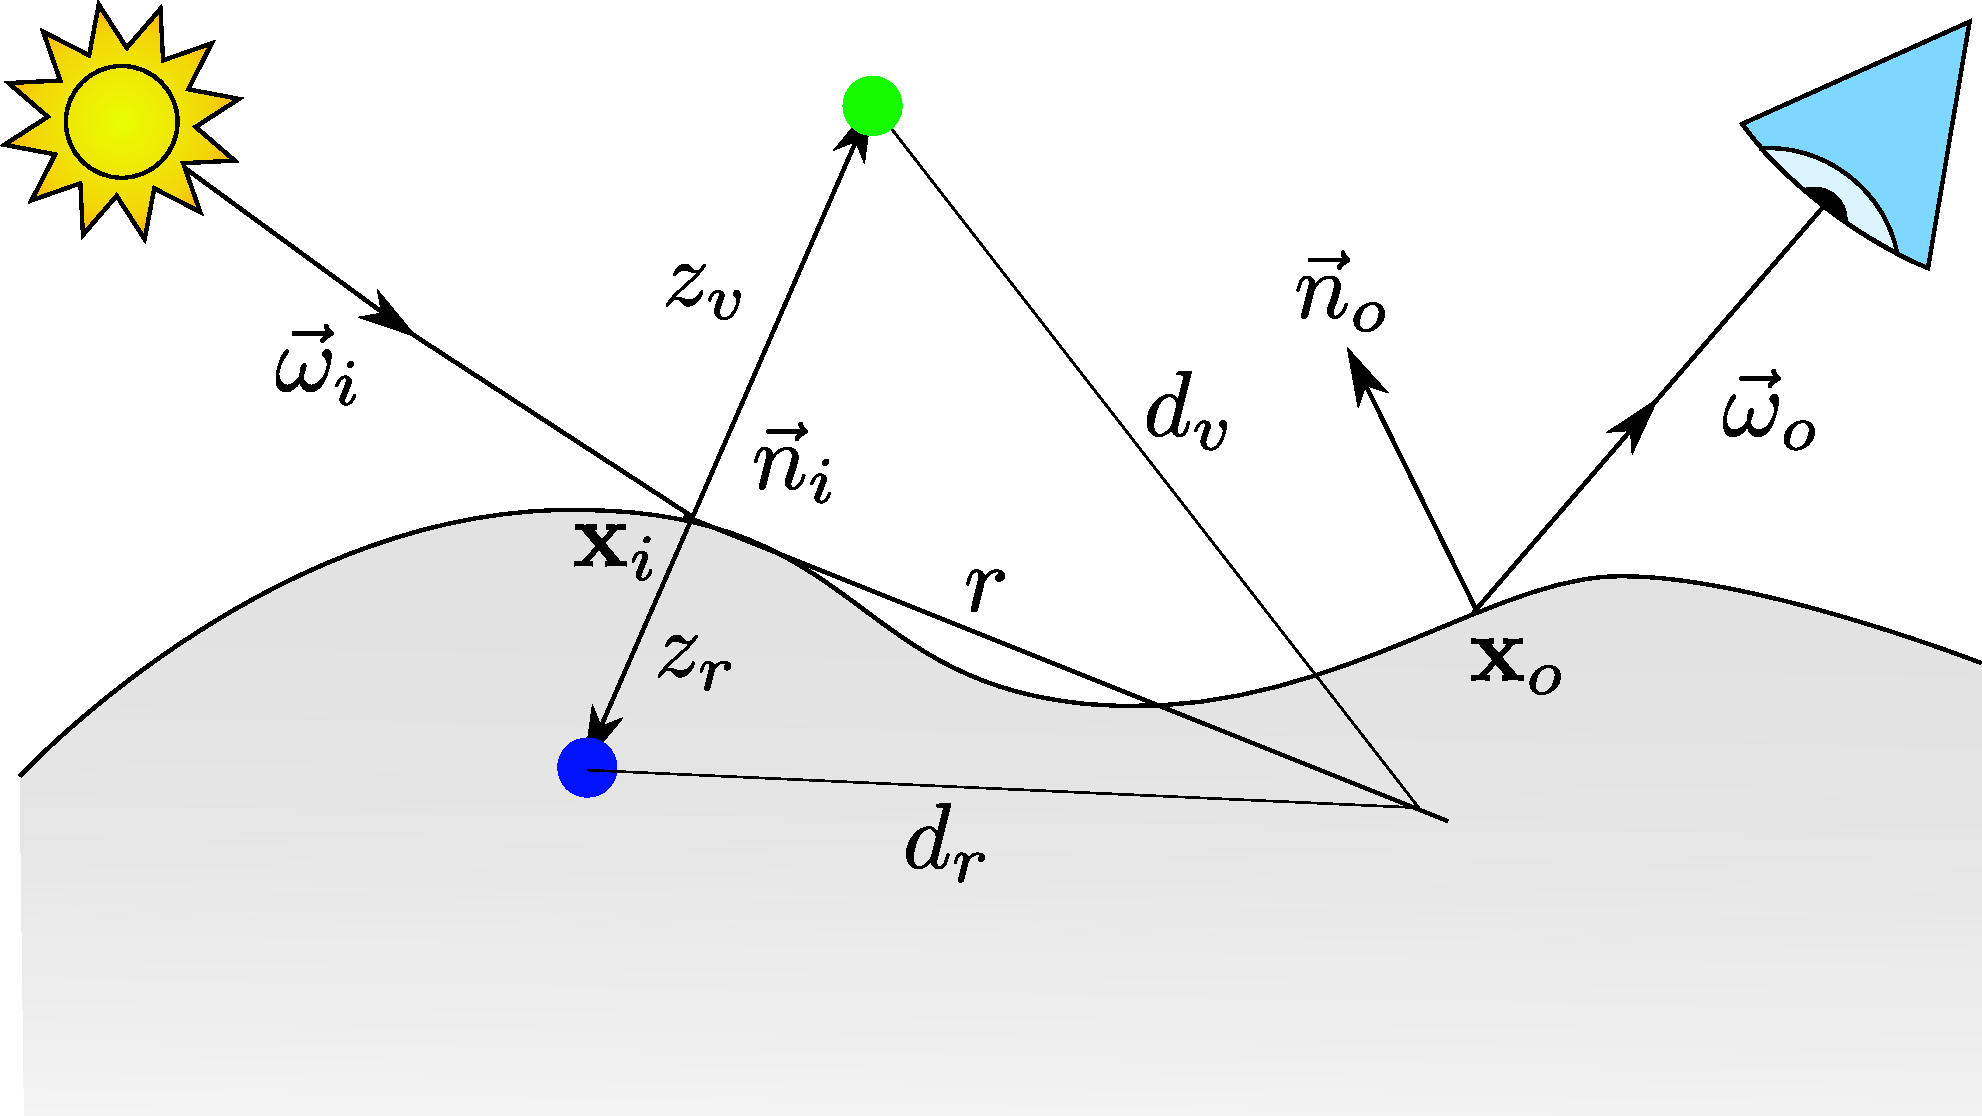
\includegraphics[width=0.55\textwidth]{jensen}
			\end{itemize}
	$$
S_d(\x_i,\vomega_i,\x_i,\vomega_o) = \frac{\alpha'}{4 \pi^2} \left[\frac{z_r (1 + \sigma_{tr} d_r) \; e^{-\sigma_{tr} d_r}}{d_r^3} + \frac{z_v (1 + \sigma_{tr} d_v) \; e^{-\sigma_{tr} d_v}}{d_v^3} \right]
$$			

\end{frame}

\begin{frame}
    \frametitle{Directional dipole}
		\vspace{0.3cm}
			\begin{itemize}
				\item \citep{IMM2013-06646} defined a new BSSRDF function that keeps the directionality of the incoming light into account
				\item The models uses a more precise diffusion approximation, that yields the following fluence formula:
				\begin{equation*}
\phi(\x, \theta) = \frac{\Phi}{4\pi D} \frac{e^{\sigma_{tr} r}}{r} \left( 1 + 3D\frac{1 + \sigma_{tr} r}{r}\cos\theta\right)
\end{equation*}
			Where we have an extra term that accounts for directionality
			\item As in the previous model, a dipole is used, but with ray sources
	\end{itemize}
\end{frame}

\begin{frame}
    \frametitle{Directional dipole}
		\vspace{0.3cm}
			\begin{itemize}
				\item Some extra corrections are needed in order to get a good boundary condition \\(modified tangent plane, distance to the real source)	\\			
				\centering
				\vspace{0.2cm}
				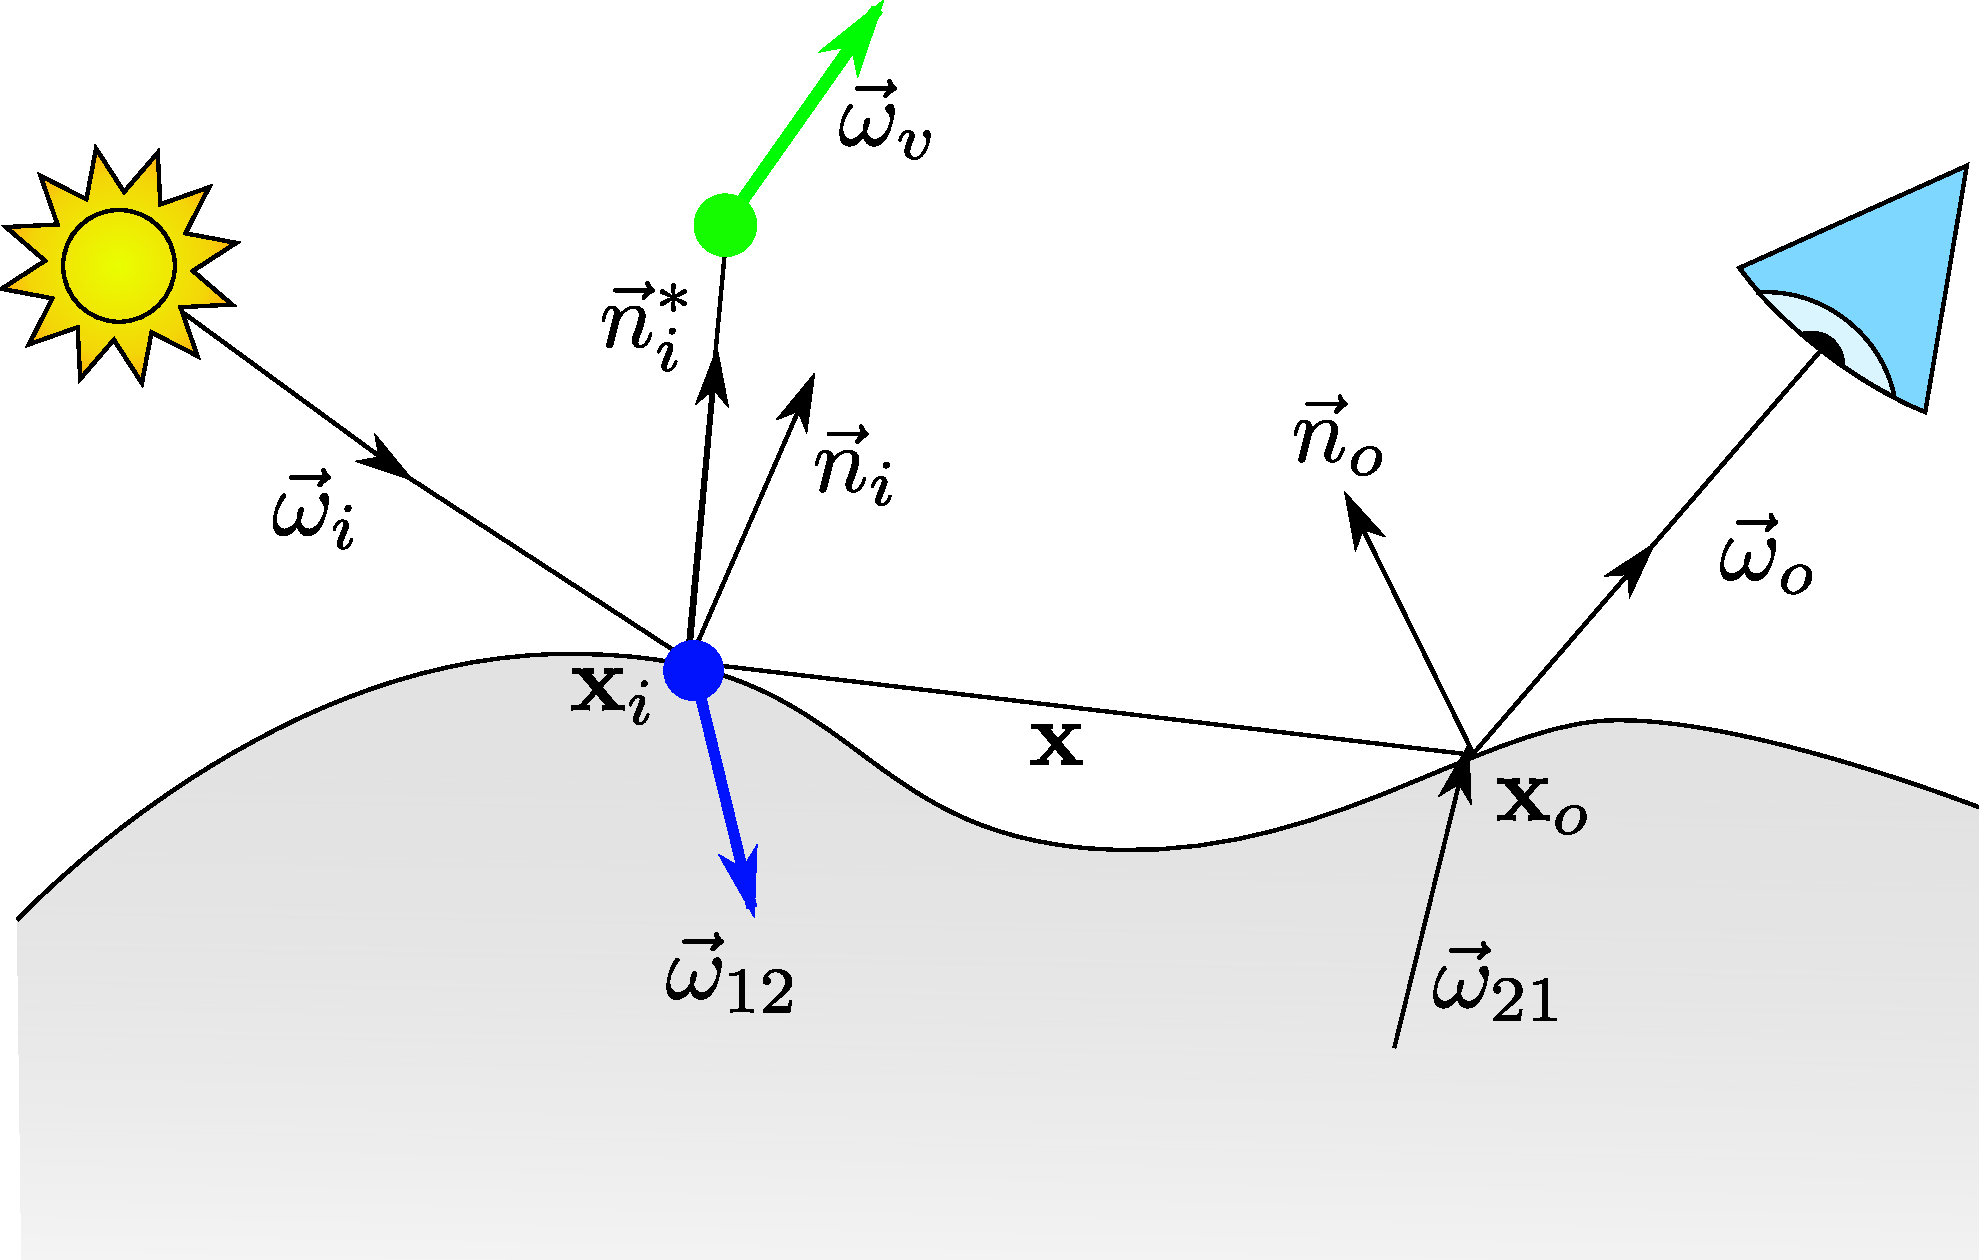
\includegraphics[width=0.55\textwidth]{jeppe}
			\end{itemize}
			$$
			S_d(\x_i, \vomega_i, \x_o) = S'_d(\x_o - \x_i, \vomega_{12}, d_r) - S'_d(\x_o - \x_v, \vomega_{v}, d_v)
			$$
\end{frame}
\section{Method}
\begin{frame}
    \frametitle{Method}
			\begin{itemize}
			\vspace{0.2cm}
			\item Scattering effects have a limited range, that depends on the scattering properties of the material (especially on $1/\sigma_{tr}$)
			\item We can then consider contributions from a disk on the surface
			\item The disk has a center point $\x_d$ and a direction $\vomega_d$
			\end{itemize}
			\centering
			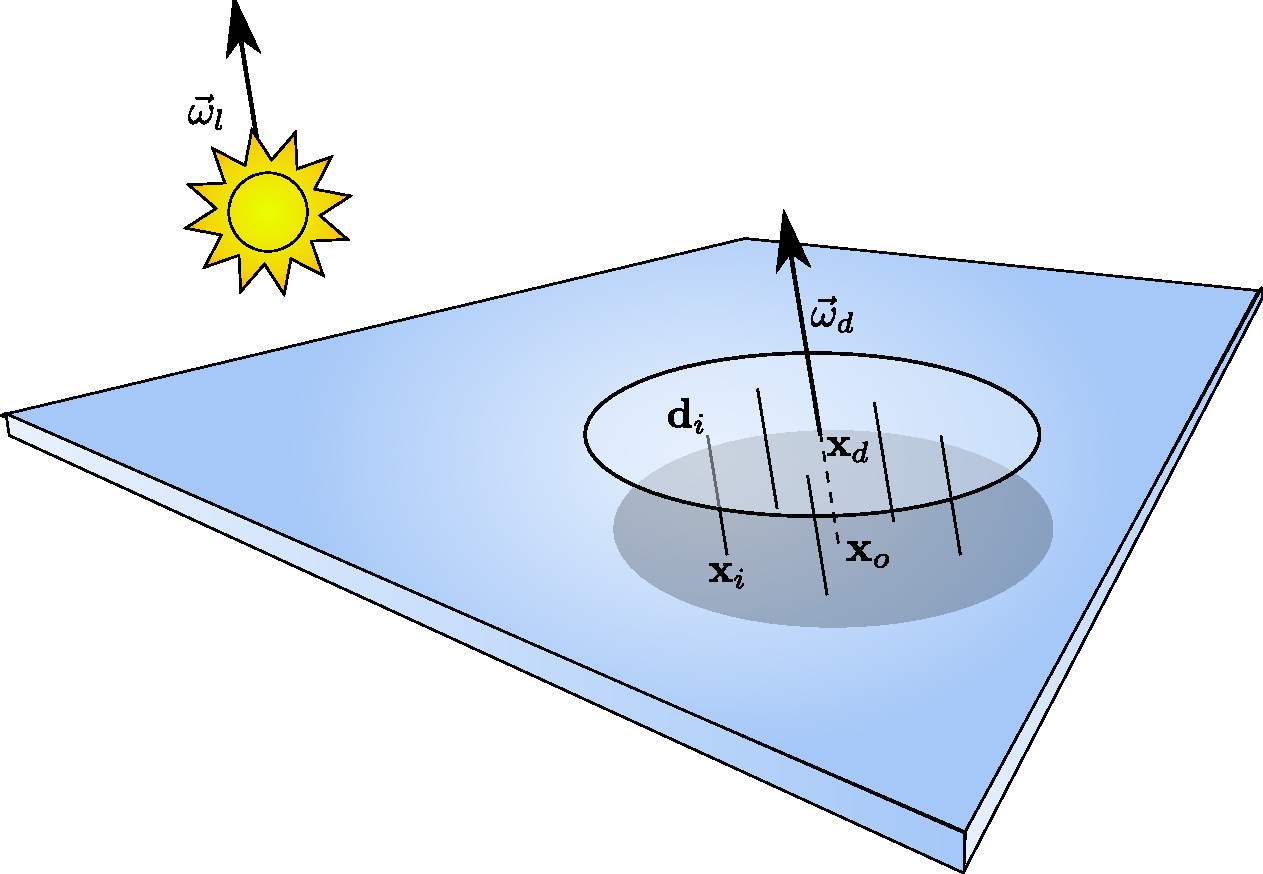
\includegraphics[width=0.55\textwidth]{disk_setup.pdf} 
\end{frame}

\begin{frame}
    \frametitle{Method}
			\begin{itemize}
			\item We place the disk oriented towards the light ($\vomega_d = \vomega_l$) and close enough to the light in order to cover the surface
			\end{itemize}
			\vspace{0.2cm}
			\begin{columns}
    \begin{column}{0.5\textwidth}
      \centering
		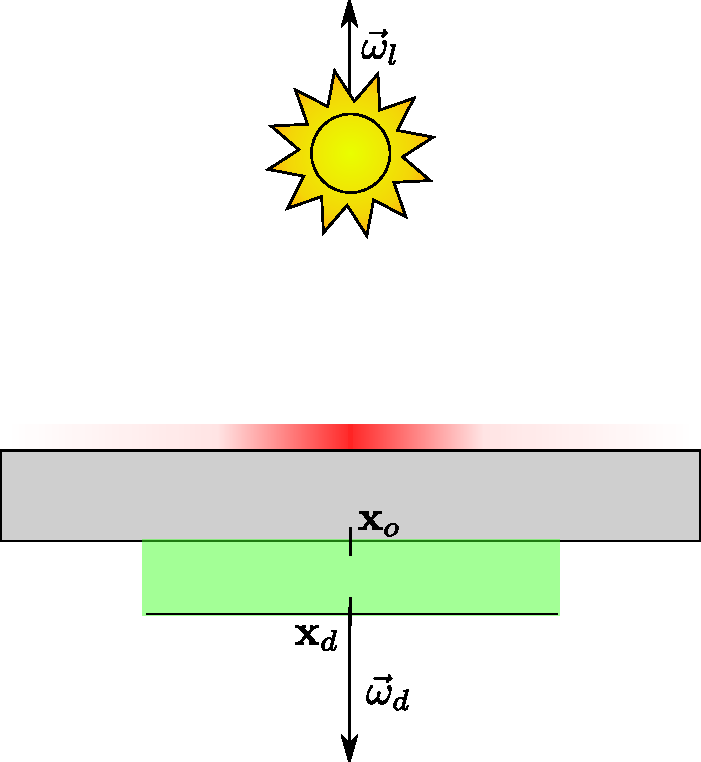
\includegraphics[width=0.8\textwidth]{distribution_wrong_1}
		\\\textit{Naïve disk placement}
				\end{column}
    \begin{column}{0.5\textwidth}
      \centering
		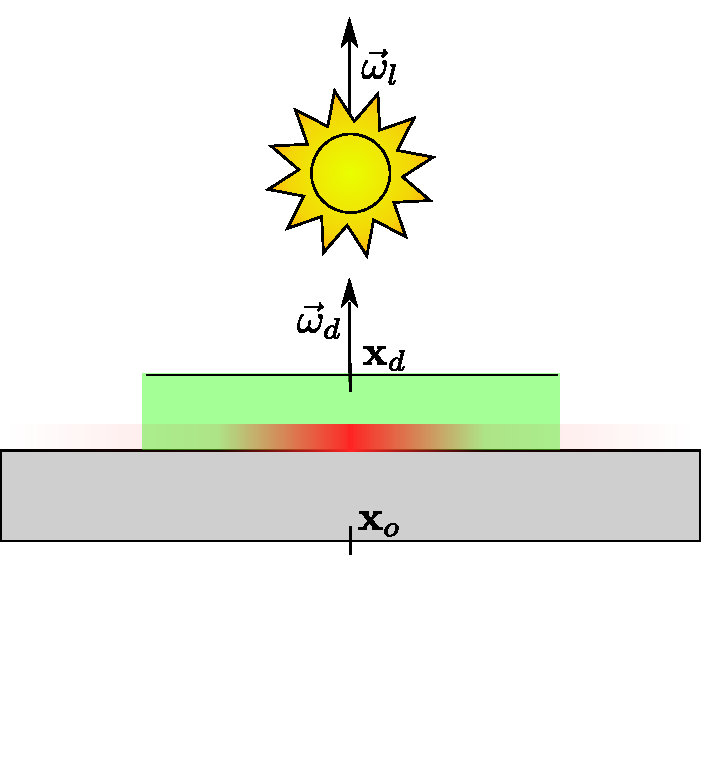
\includegraphics[width=0.8\textwidth]{distribution_wrong_2}
		\\\textit{Our disk placement}
    \end{column}
​  \end{columns}

\end{frame}

\begin{frame}
    \frametitle{Method}
			\begin{itemize}
			\item Given these assumptions on the disk, we discretize the rendering equation
			\item We distribute the samples on the disk exponentially with distribution $pdf(x) = \sigma_{tr} \;e^{-\sigma_{tr}x}$
			\end{itemize}
				$$
				L_o(\x_o,\vomega_o) = L_d \frac{A_c}{N} \sum_{i = 1}^N S(\x_i, \vomega_l, \x_o, \vomega_o)  e^{\sigma_{tr} r_i}
				$$
				\vspace{-0.6cm}
				\centering
				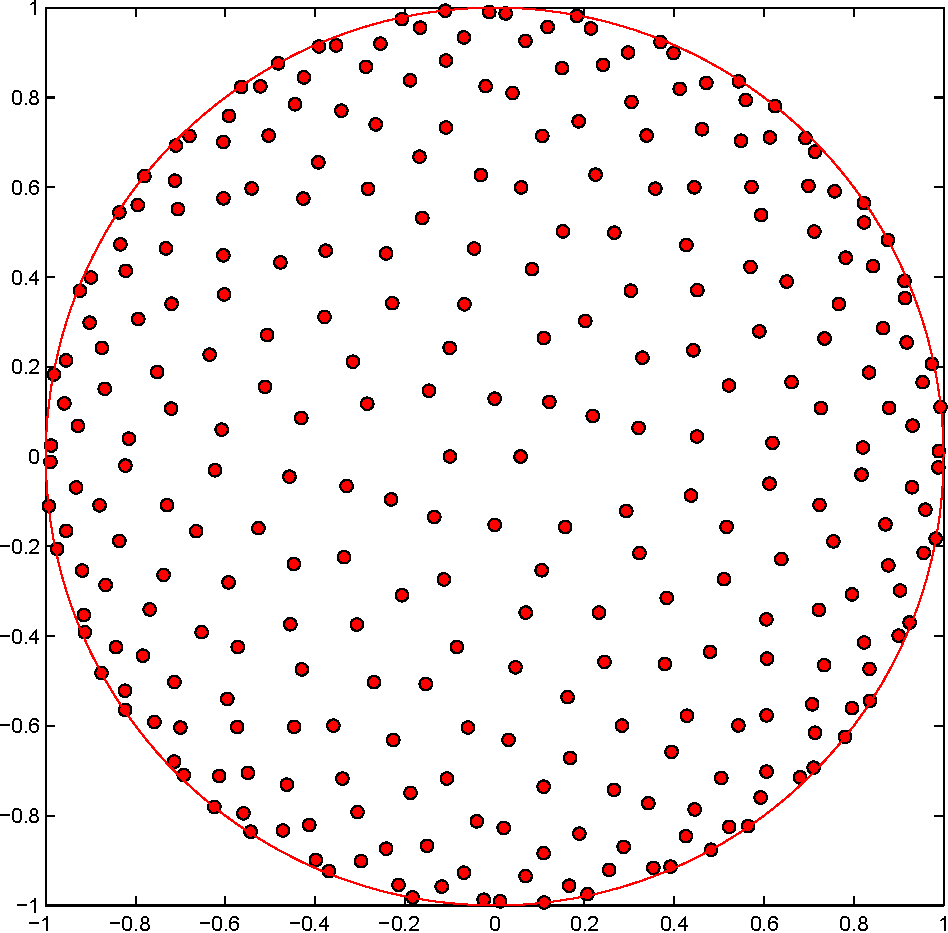
\includegraphics[width=0.3\textwidth]{halton.pdf} \hspace{1cm}	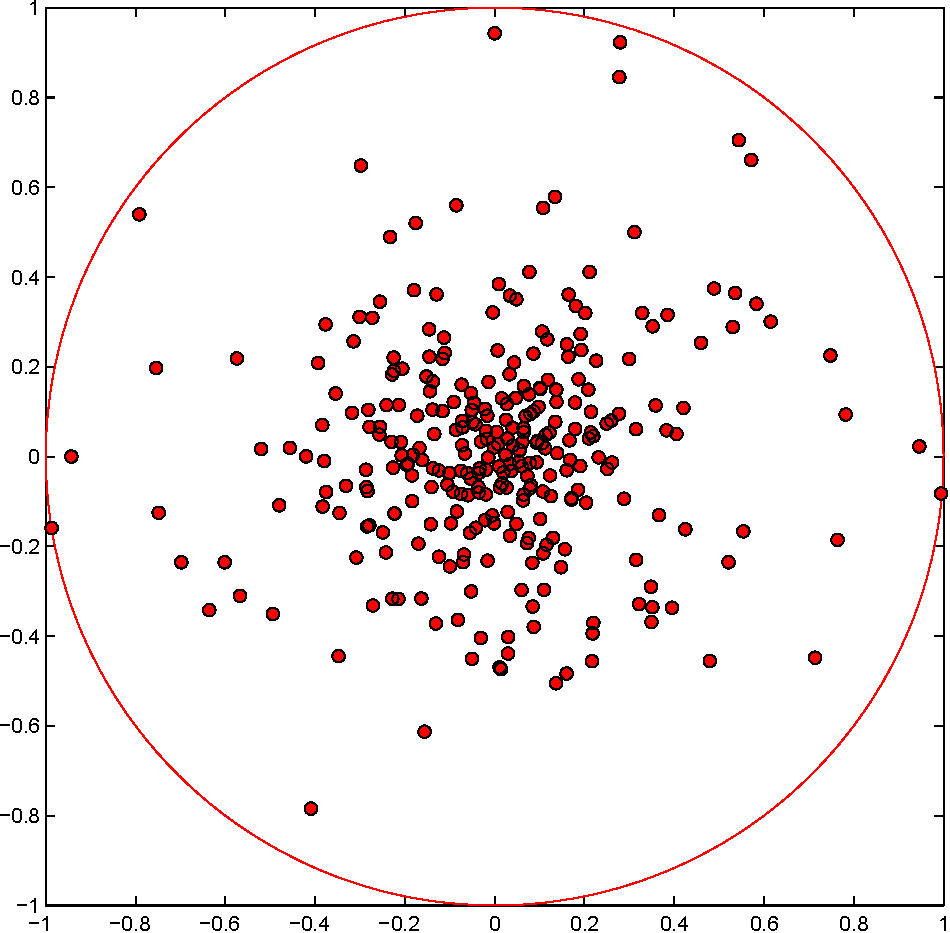
\includegraphics[width=0.3\textwidth]{halton_exp.pdf}

\end{frame}

\section{Implementation}
\begin{frame}
    \frametitle{Implementation (step 1)}
			\begin{itemize}
			\item We render the scene from the light point of view (as in \emph{shadow mapping})
			\item We store positions and normals in a texture, the \emph{light map}
			\item We get the closest points to light
			\end{itemize}
			\centering
			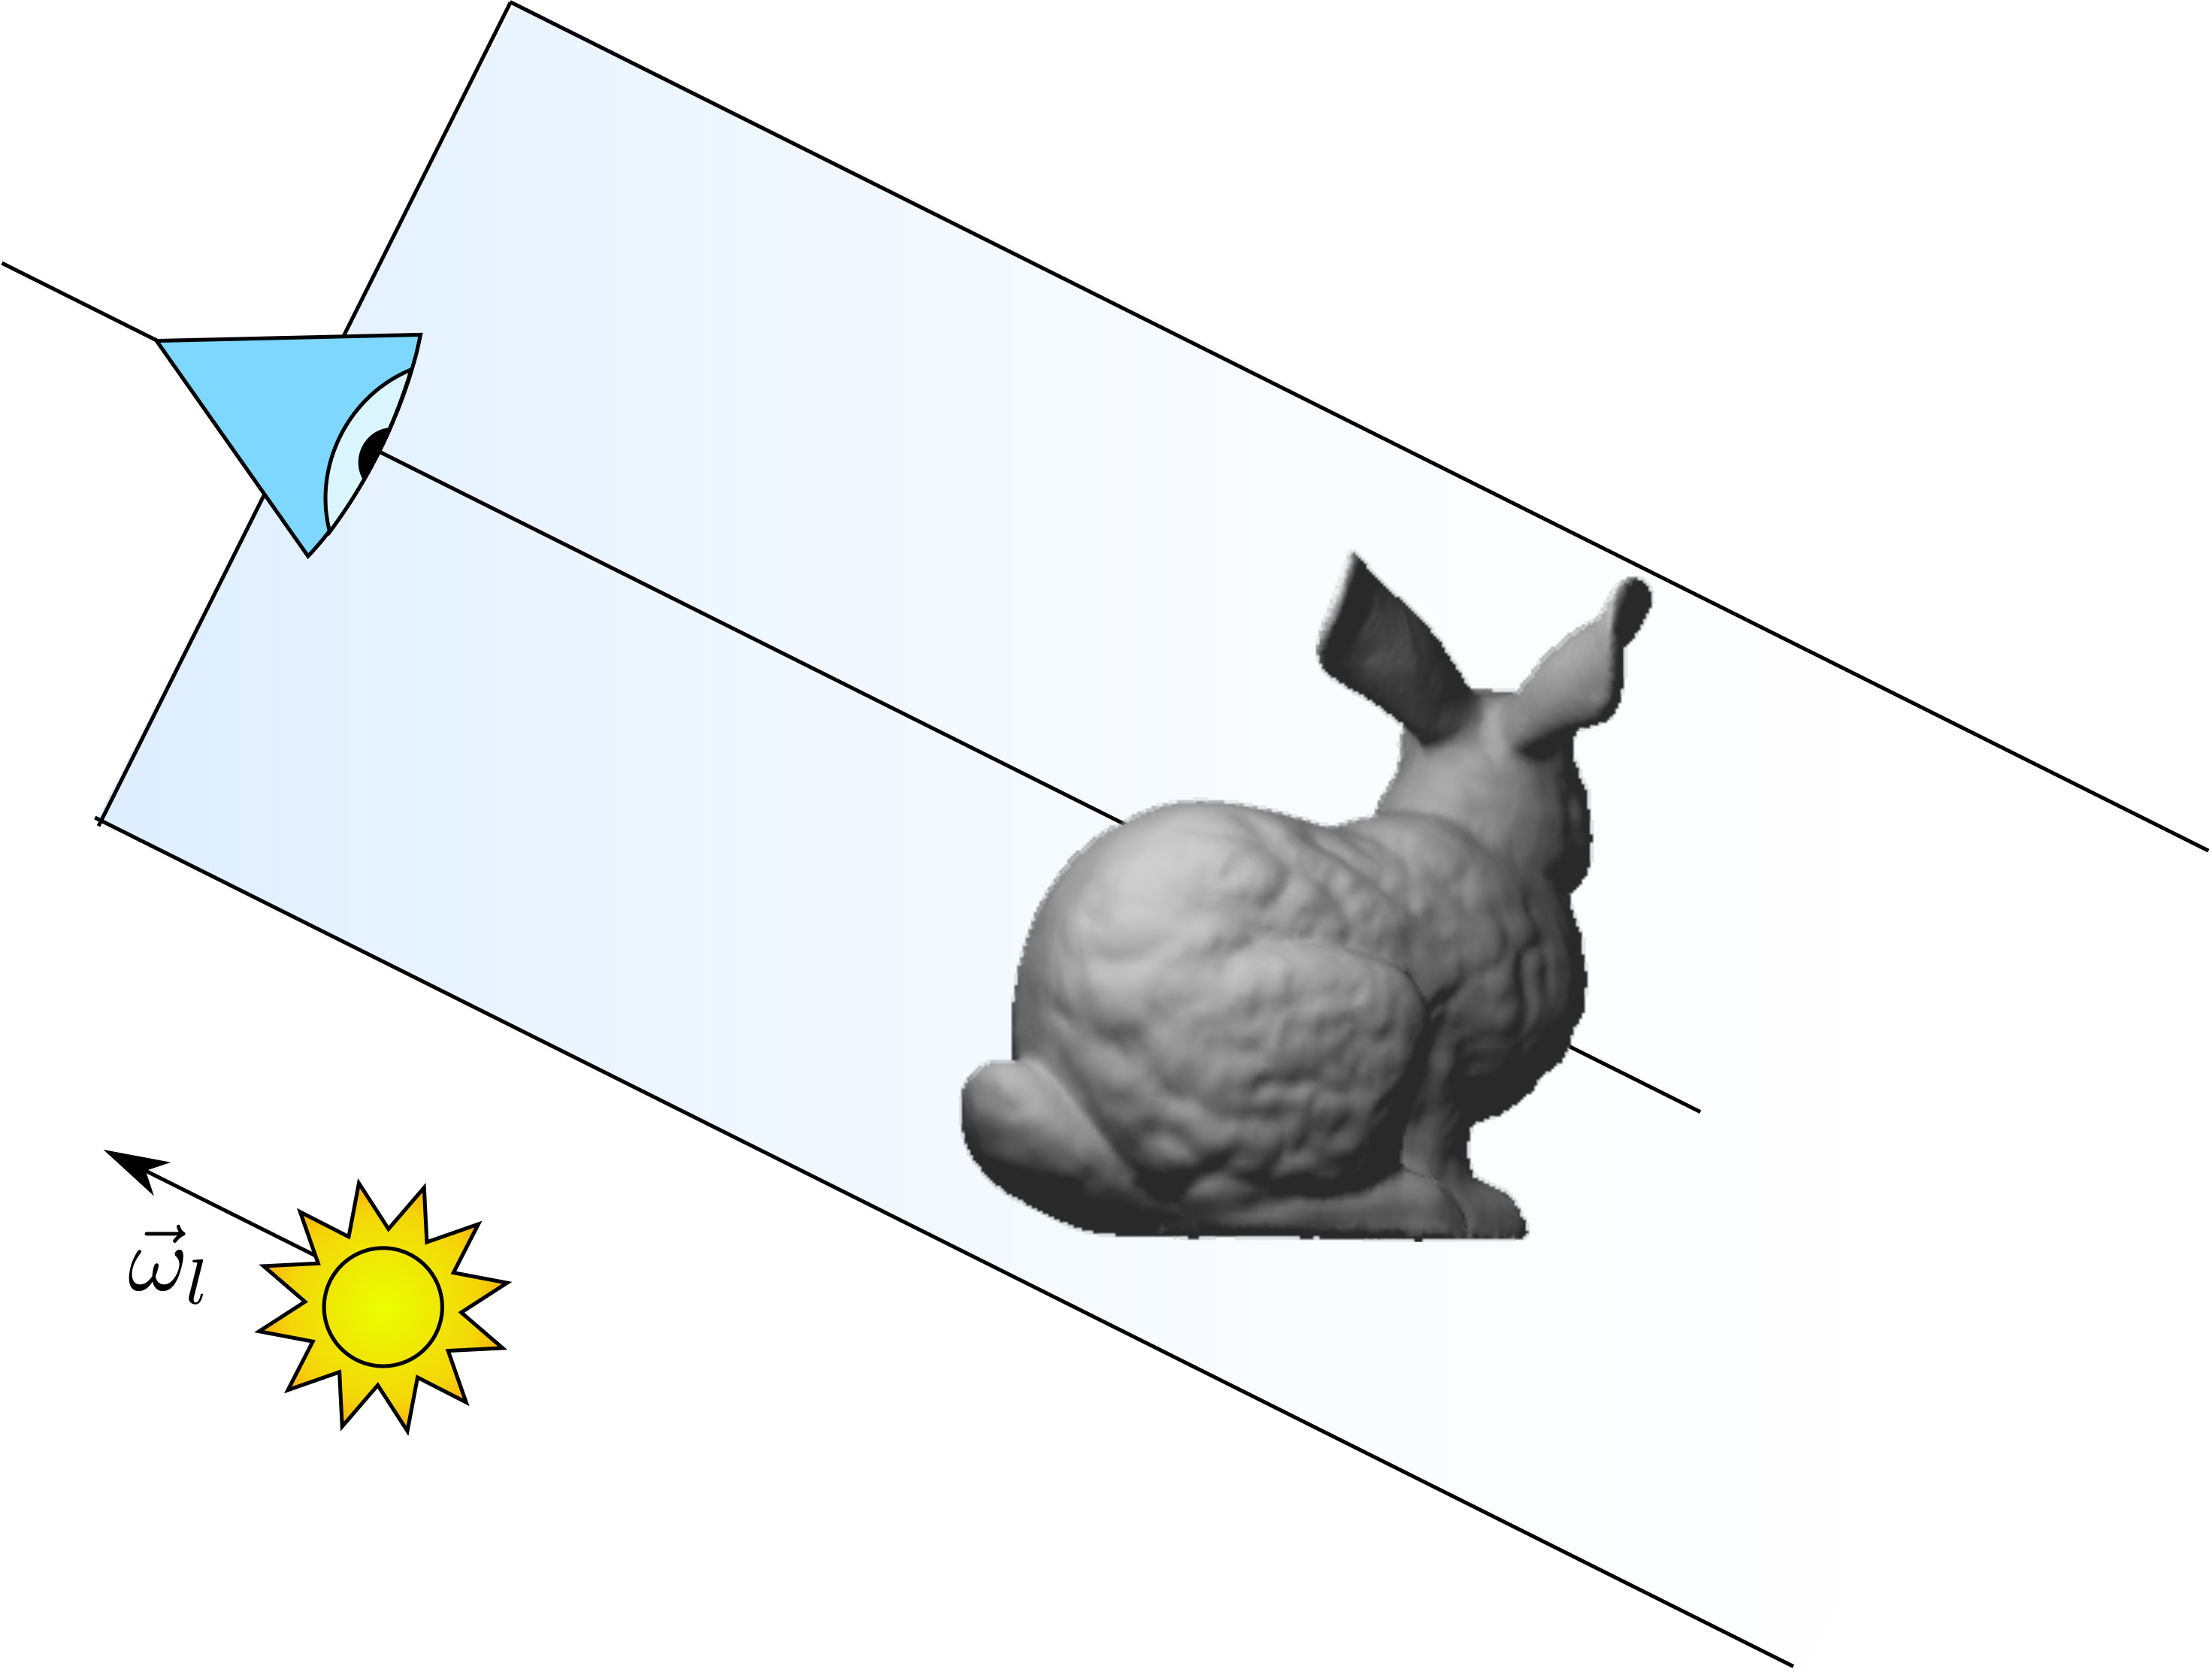
\includegraphics[width=0.5\textwidth]{step1.jpg} 
\end{frame}

\begin{frame}
    \frametitle{Implementation (step 2)}
			\begin{itemize}
			\item We render the object from a certain number of directions in the \emph{radiance map}
			\item The directions can be chosen randomly or placed by the artist
			\item For each pixel we sample the points from the light map and sum up the BSSRDF contribution
			\end{itemize}
			\centering
			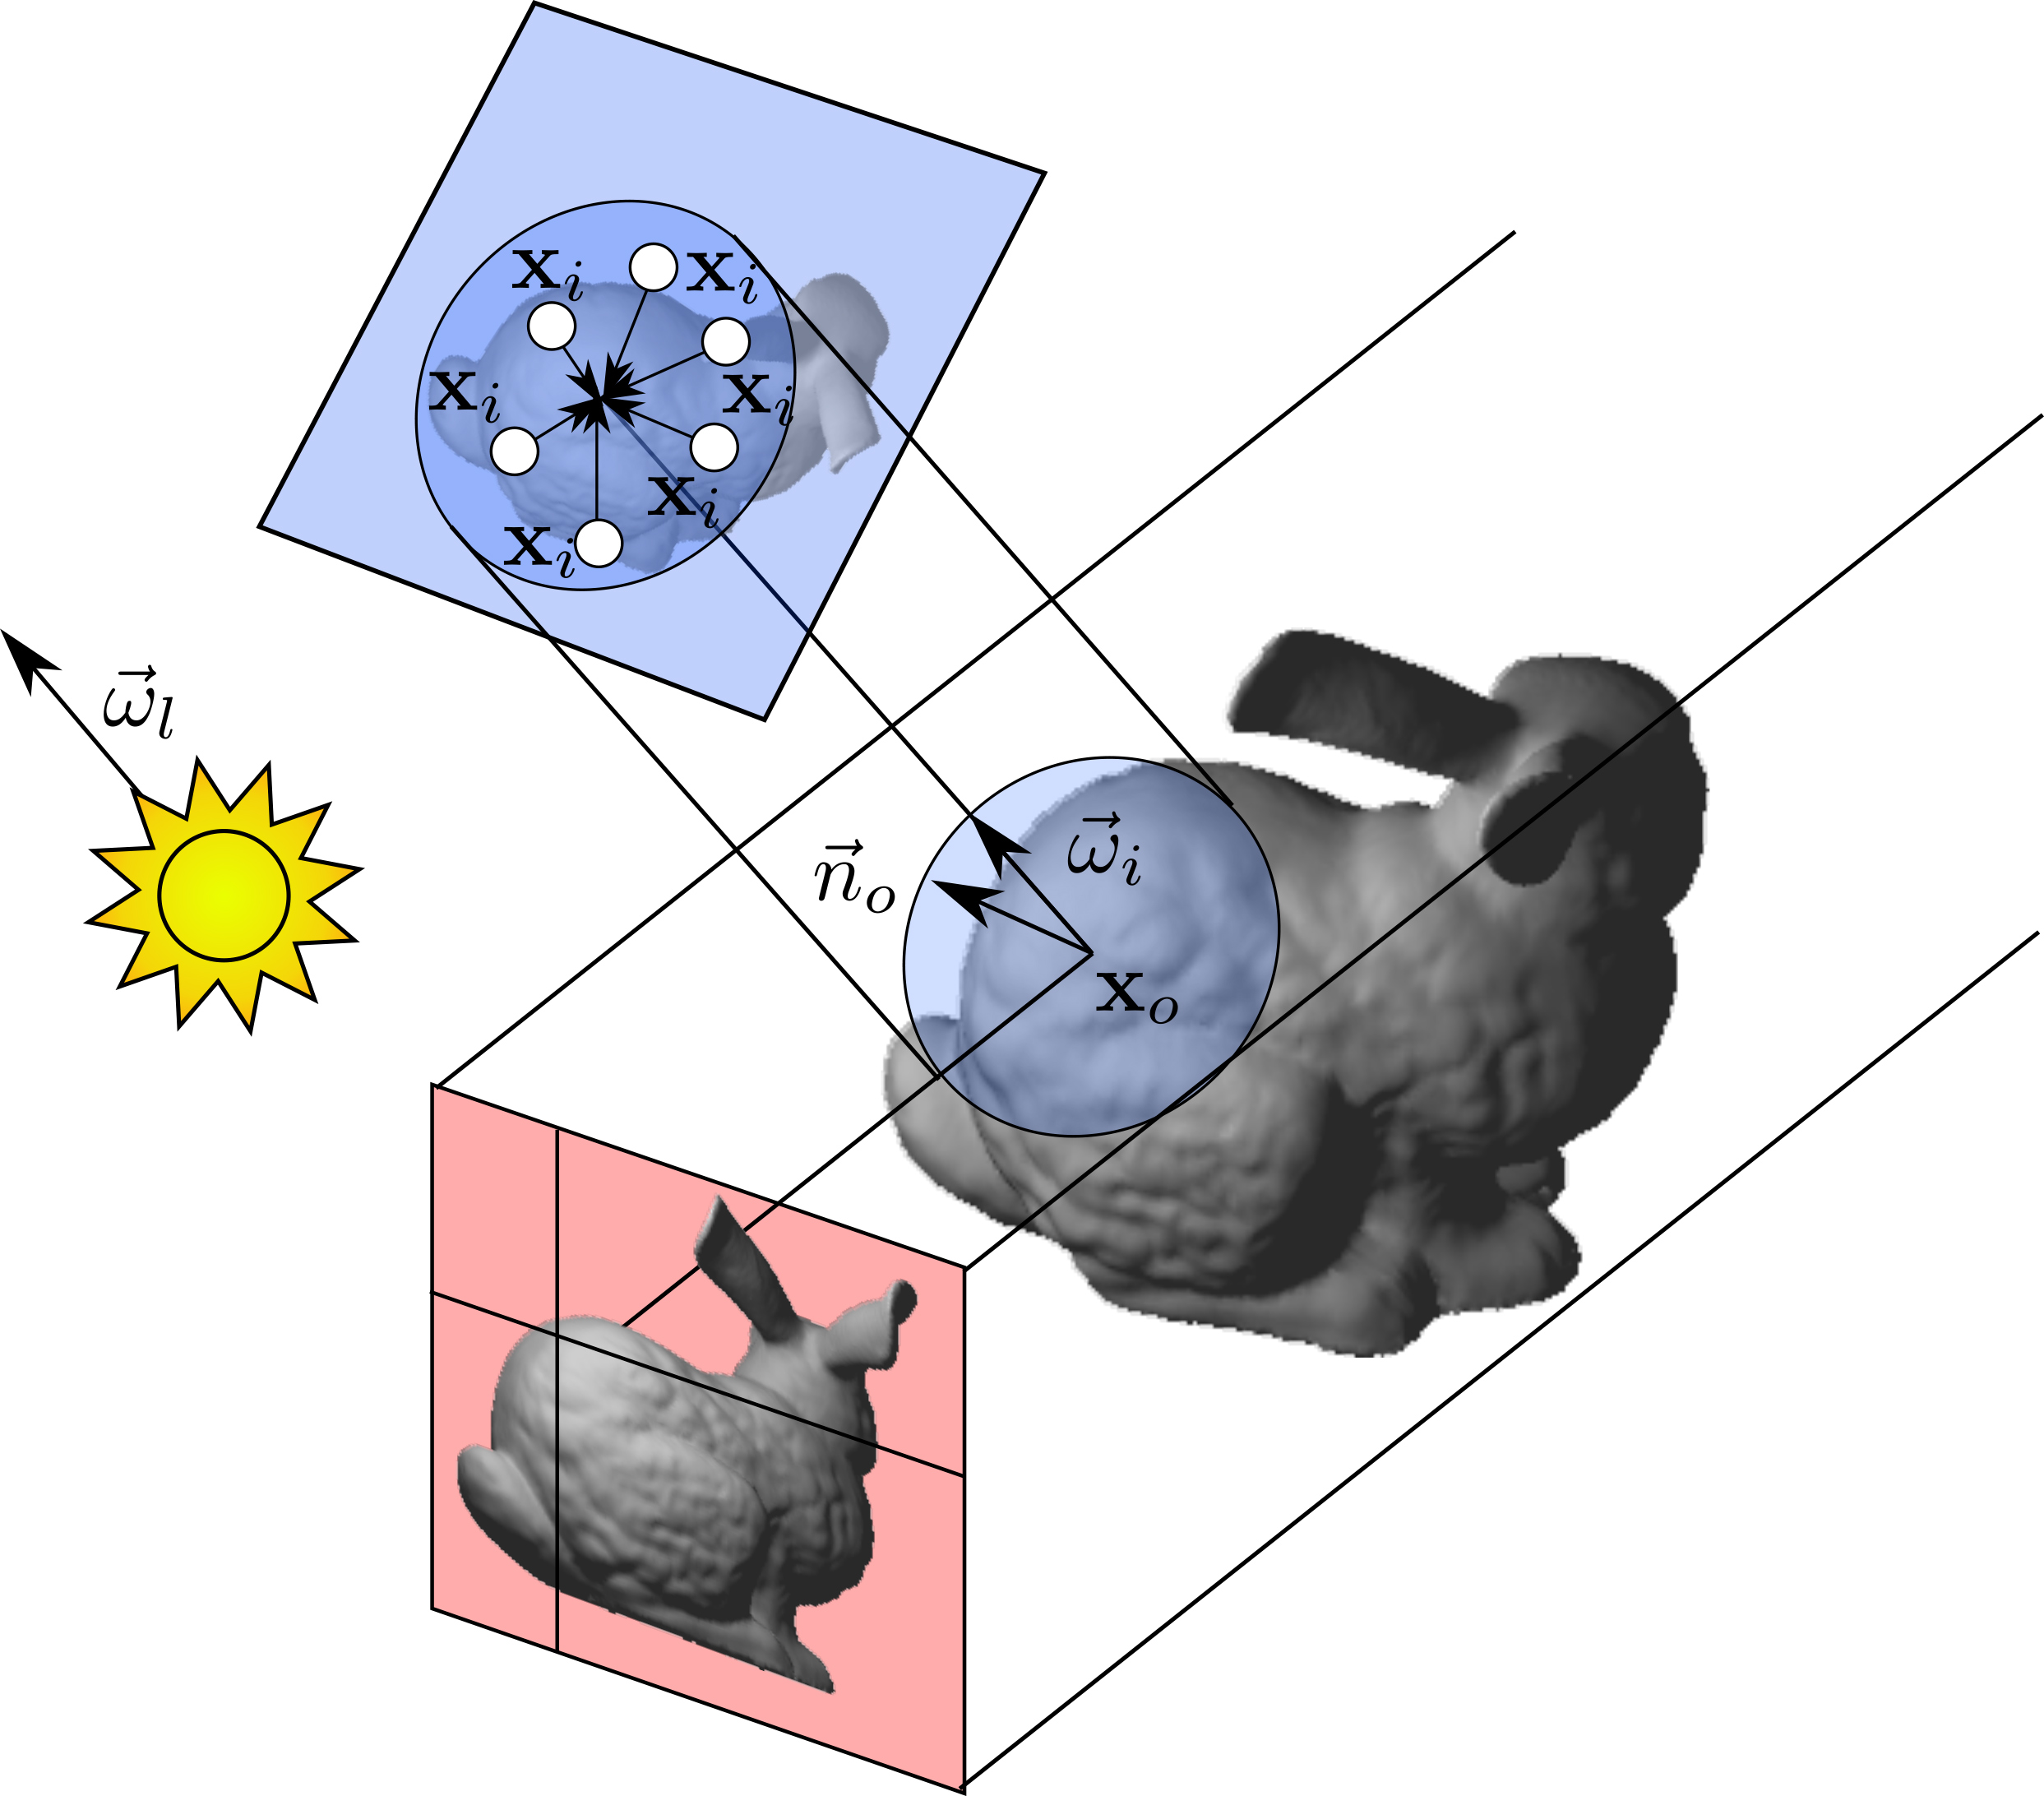
\includegraphics[width=0.4\textwidth]{step2.jpg} 
\end{frame}

\begin{frame}
    \frametitle{Implementation (step 3)}
			\begin{itemize}
			\item We finally sample the radiance map to get the single contribution for a point on the surface
			\item The result is averaged over the directions from which the surface point is visible
			\end{itemize}
			\centering
			\vspace{-0.5cm}
			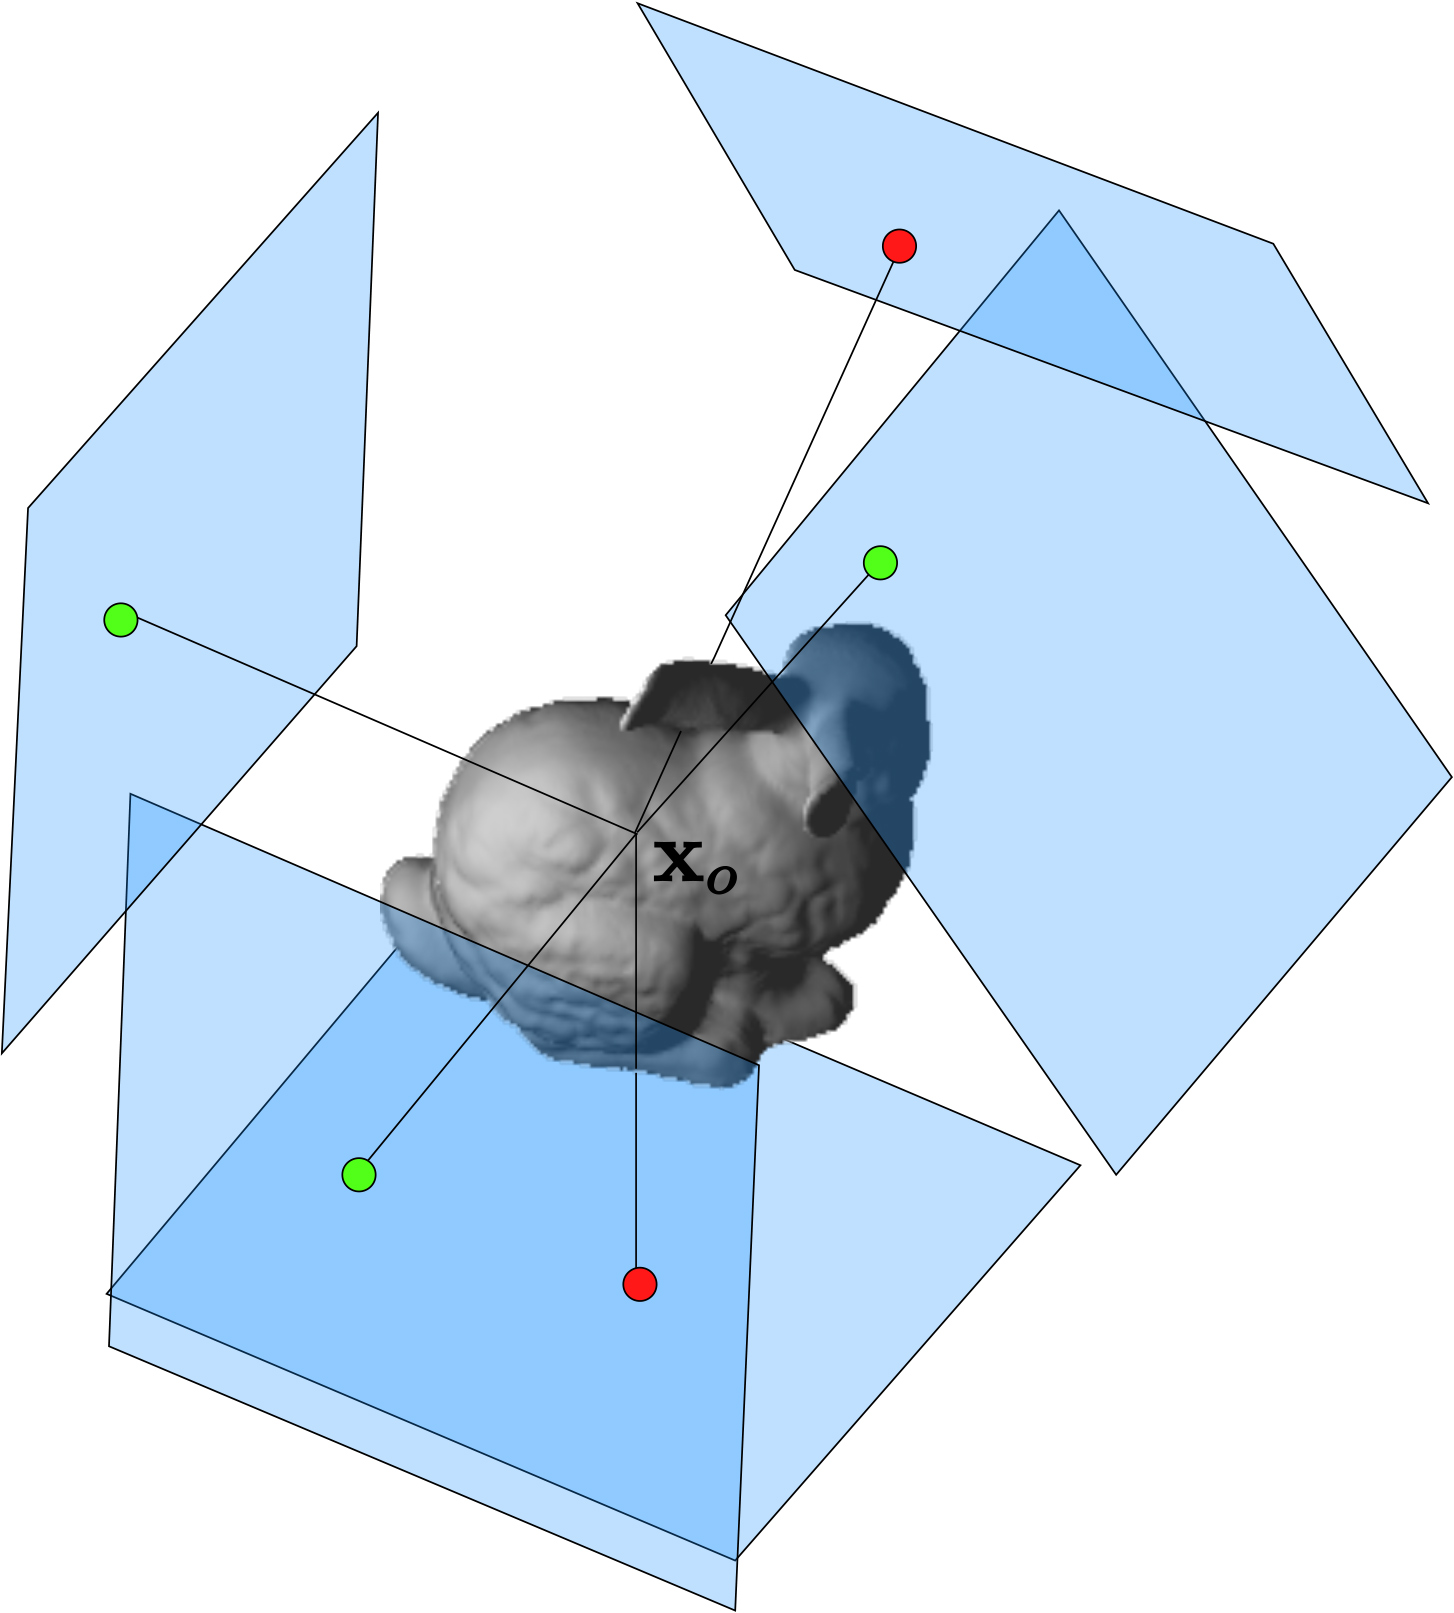
\includegraphics[width=0.4\textwidth]{step3.jpg} 
\end{frame}

\begin{frame}
    \frametitle{Implementation}
\begin{figure}
\vspace{0.3cm}
\centering
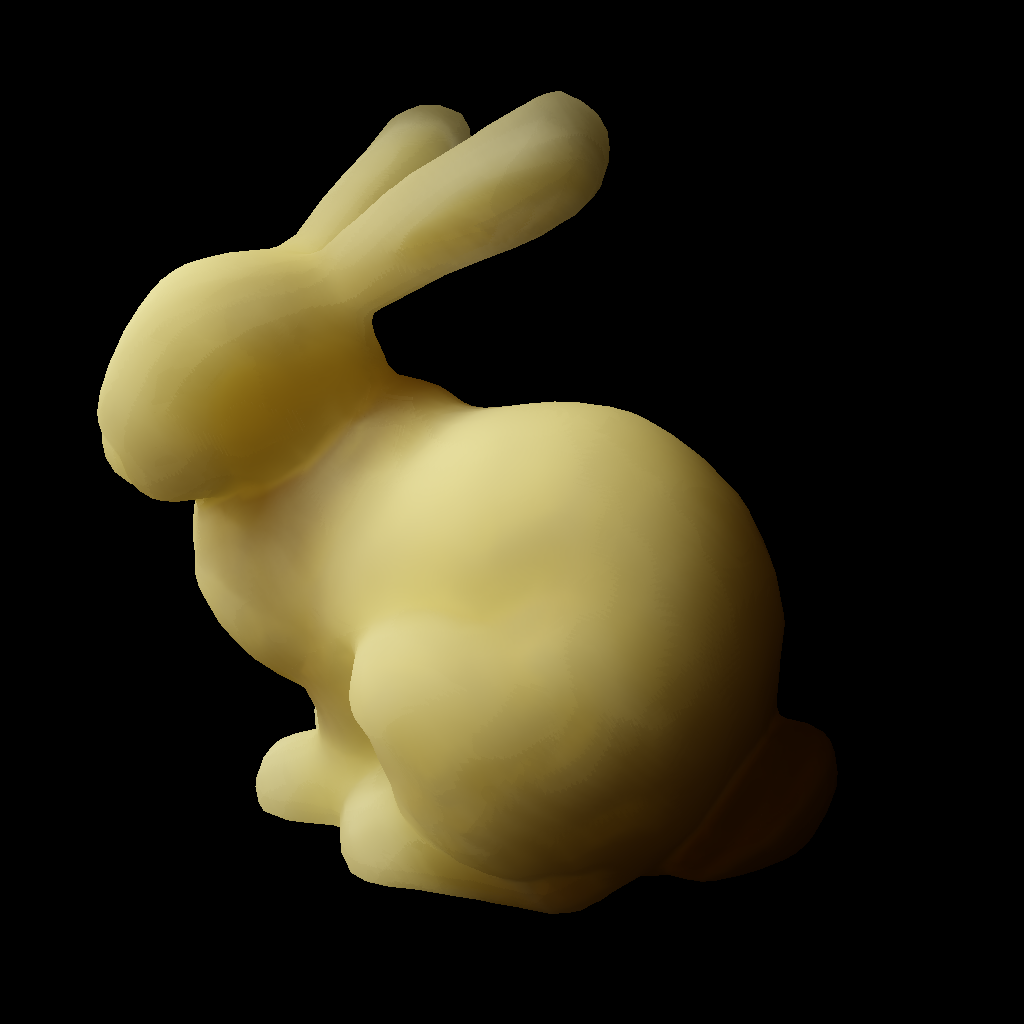
\includegraphics[width=0.55 \textwidth]{bunny}
\vspace{-0.3cm}
\caption{Stanford Bunny, potato material. Note the self shadowing automatically generated by the algorithm.}
\end{figure}
\end{frame}

\begin{frame}
    \frametitle{Advantages}
\begin{itemize}
	\item Accounts for self shadowing and self occlusion
	\item Accounts for occlusion between different objects
	\item Directly coupled with an existing shadow mapping pipeline
	\item Low memory requirements compared to a full voxelization
	\item The final step can be adapted to forward and deferred shading pipelines
\end{itemize}
\end{frame}


\begin{frame}
    \frametitle{Disadvantages}
\begin{itemize}
	\item Noisy result, that need to be either accumulated or blurred in order to achieve a smooth result
	\item Cameras that cover the surface need to be placed manually (to avoid tearing)
	\item Inherited problems from shadow mapping (constant shadow bias)
\end{itemize}
	\centering
	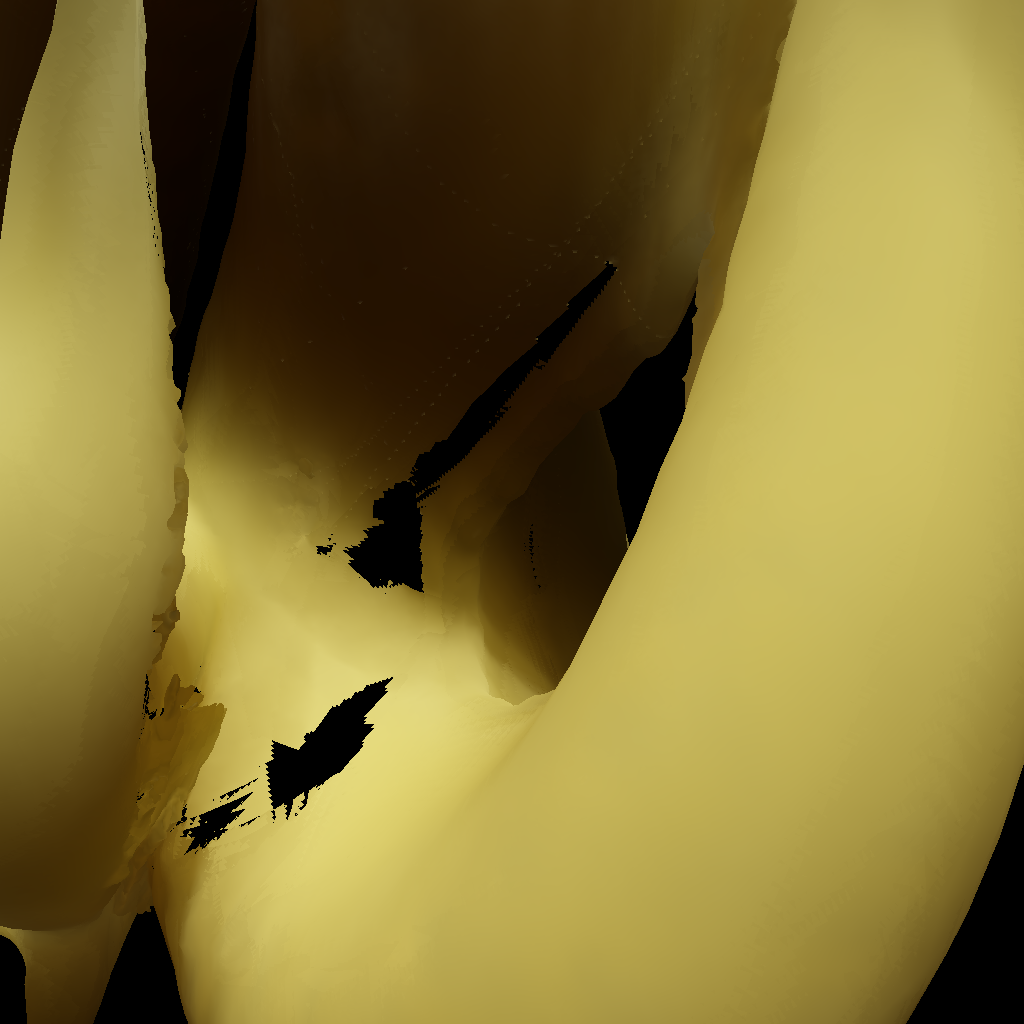
\includegraphics[width=0.3 \textwidth]{tearing}
\end{frame}

\begin{frame}
    \frametitle{Extensions}
\begin{itemize}
\vspace{0.4cm}
	\item \texttt{Multiple lights} \\ We sum the contribution of multiple lights in the shader
	\item \texttt{Point lights} \\ We scale the incoming intensity by a inverse square distance term	
\end{itemize}
\begin{columns}
    \begin{column}{0.45\textwidth}
      \centering
		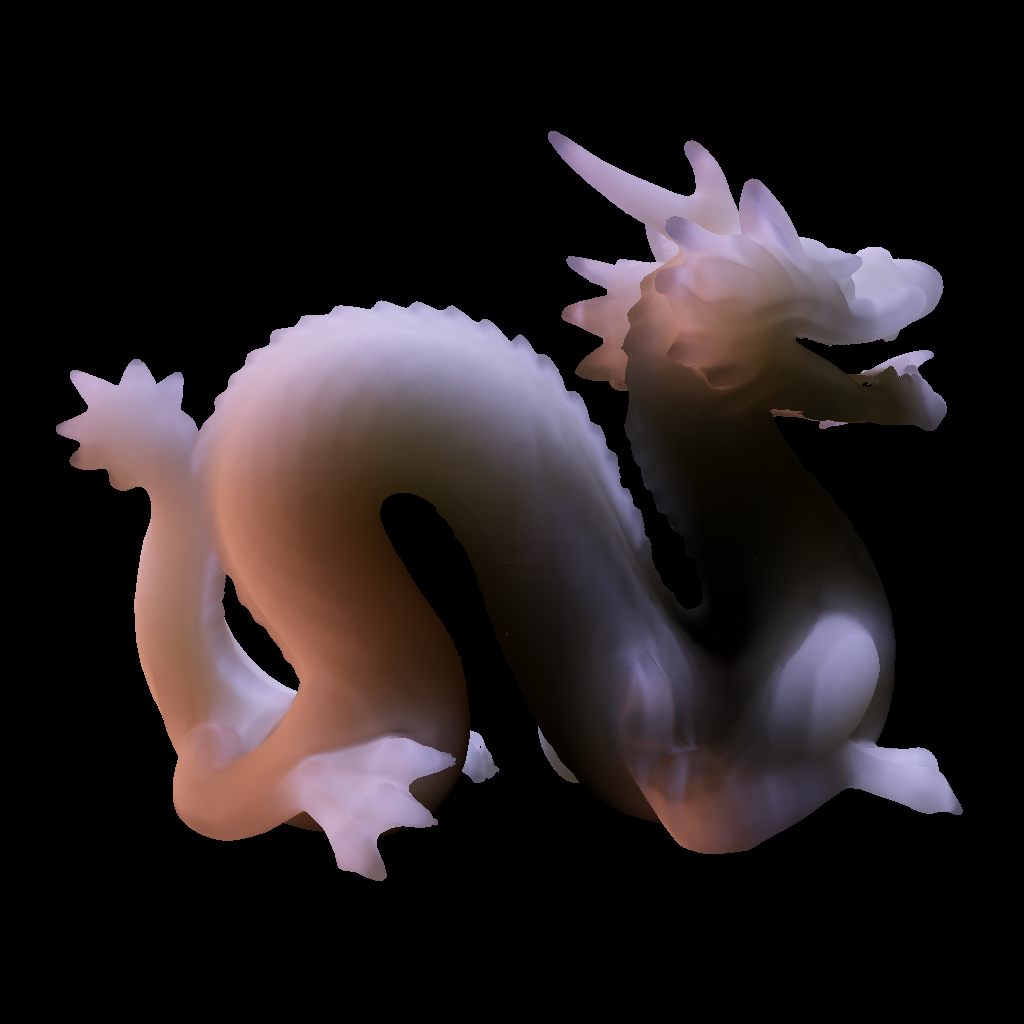
\includegraphics[width=0.9\textwidth]{multiple}
				\end{column}
   \begin{column}{0.45\textwidth}
      \centering
		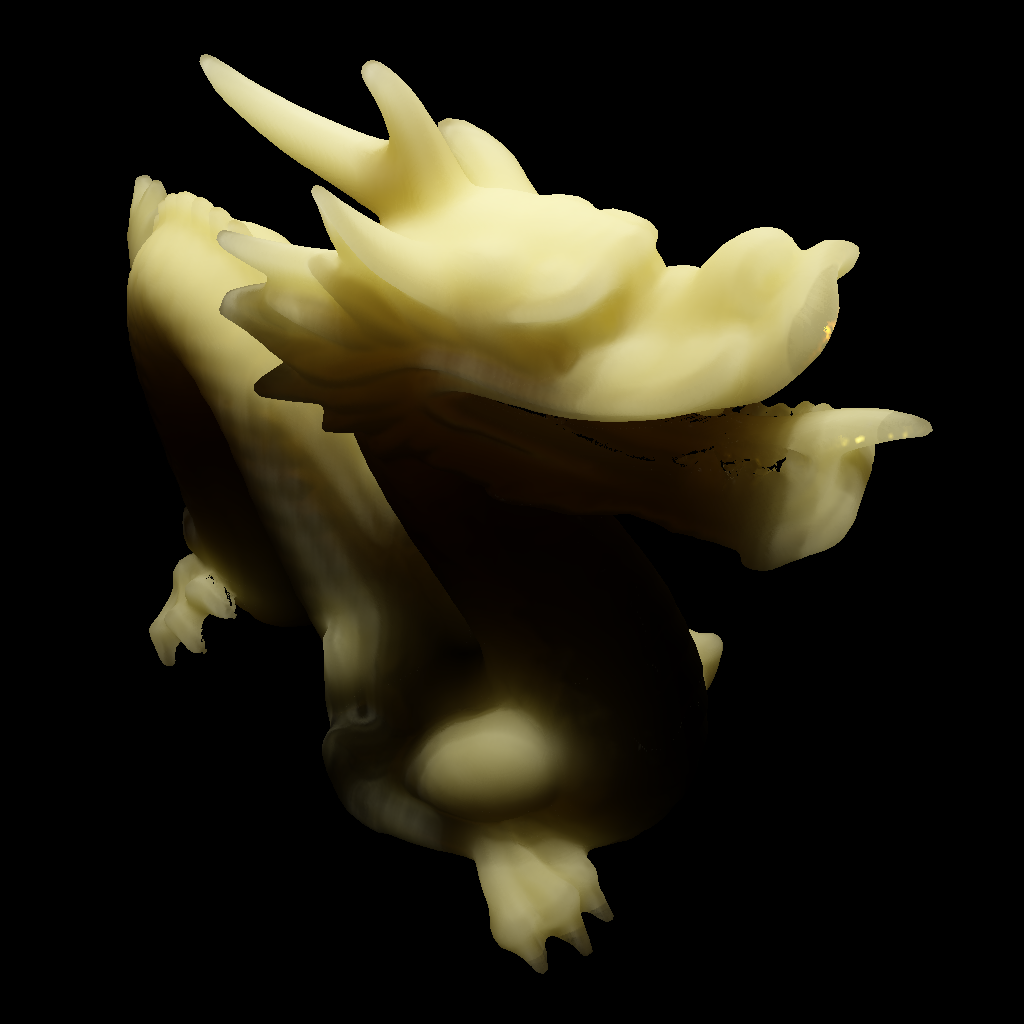
\includegraphics[width=0.9\textwidth]{point}
				\end{column}
​  \end{columns}
\end{frame}

\begin{frame}
    \frametitle{Environment lighting}
\begin{itemize}
	\item We simulate it using 16 directional lights 
	\item We choose "random" points on a light map 
	\item The distribution chosen accounts to make the points fall in areas with high radiance
\end{itemize}
      \centering
		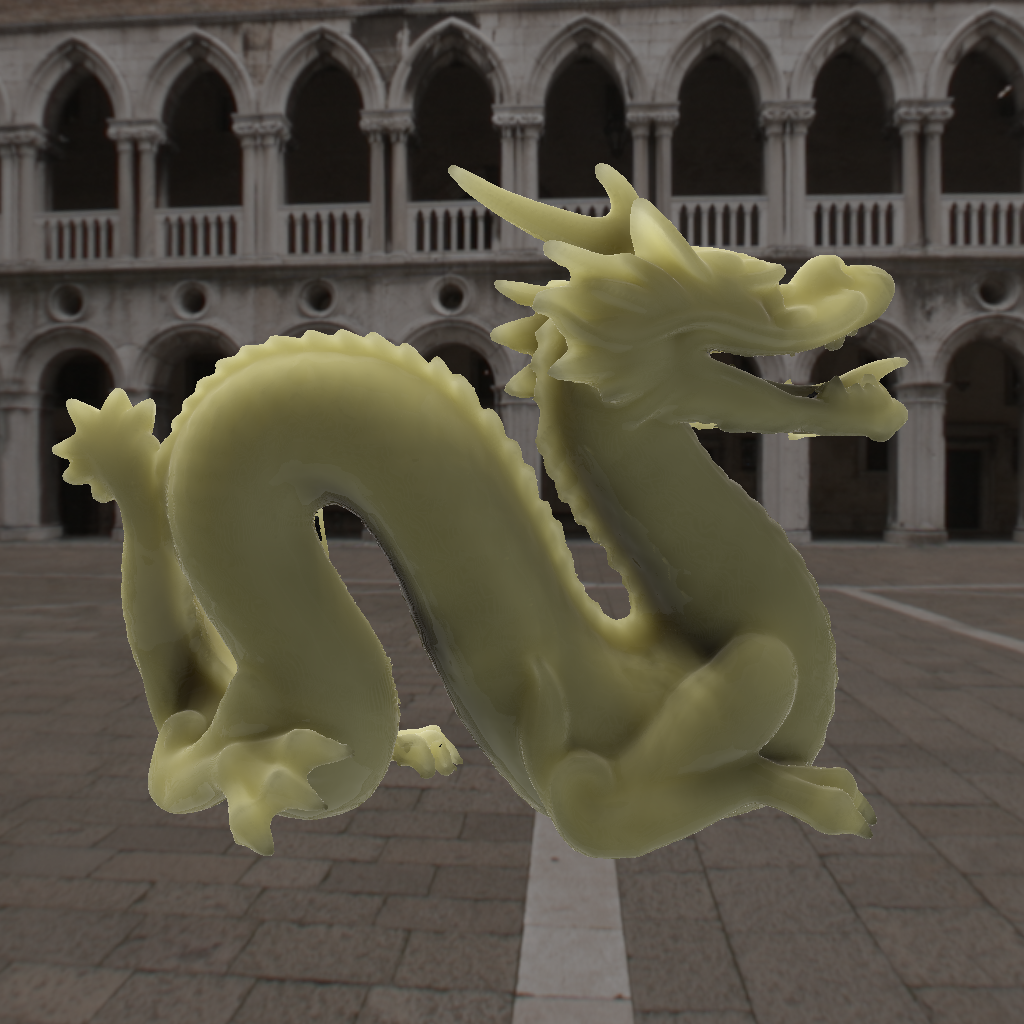
\includegraphics[width=0.4\textwidth]{skymap}
\end{frame}

\section{Results}
\begin{frame}
    \frametitle{Results (quality)}
		\begin{figure}
\centering
\subfloat[{$\ N = 100$}]{
  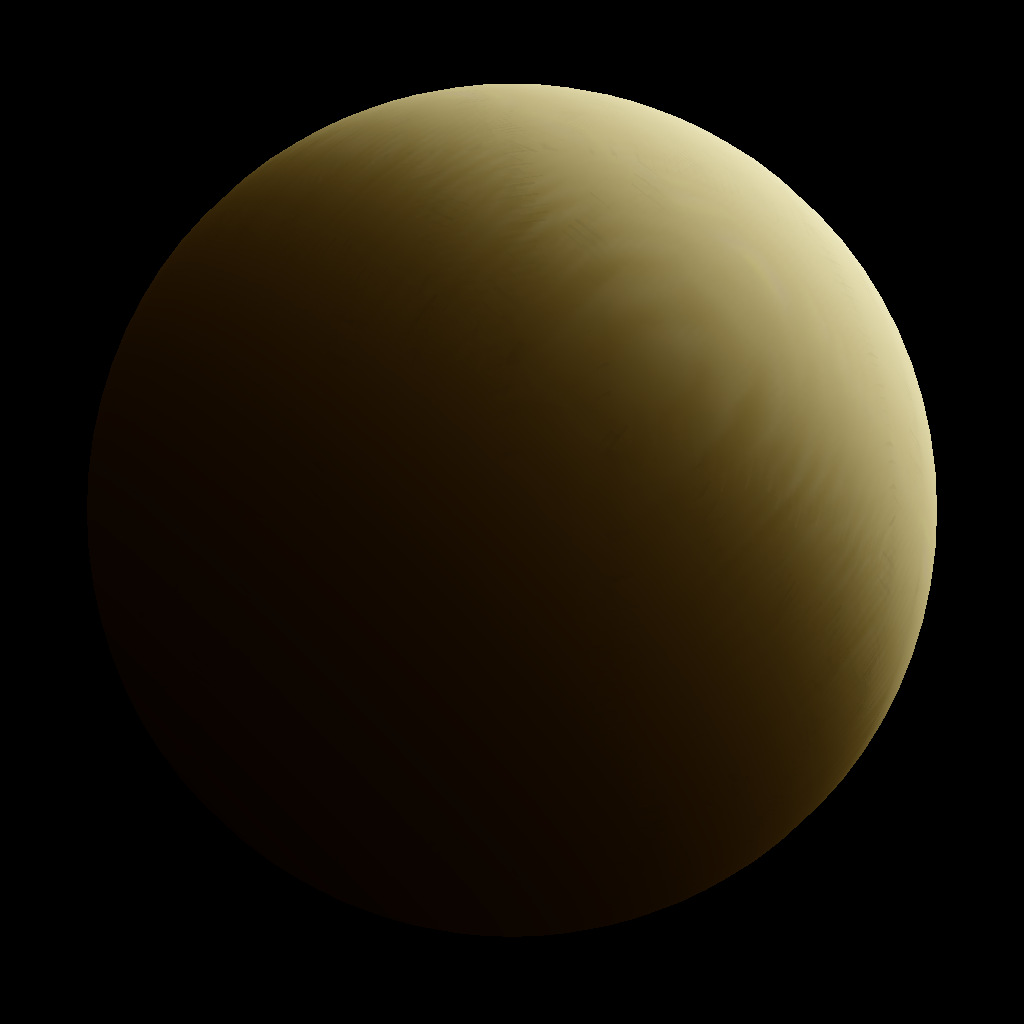
\includegraphics[width=0.25 \textwidth]{p100}
}
\subfloat[{$\ N = 1000$}]{
  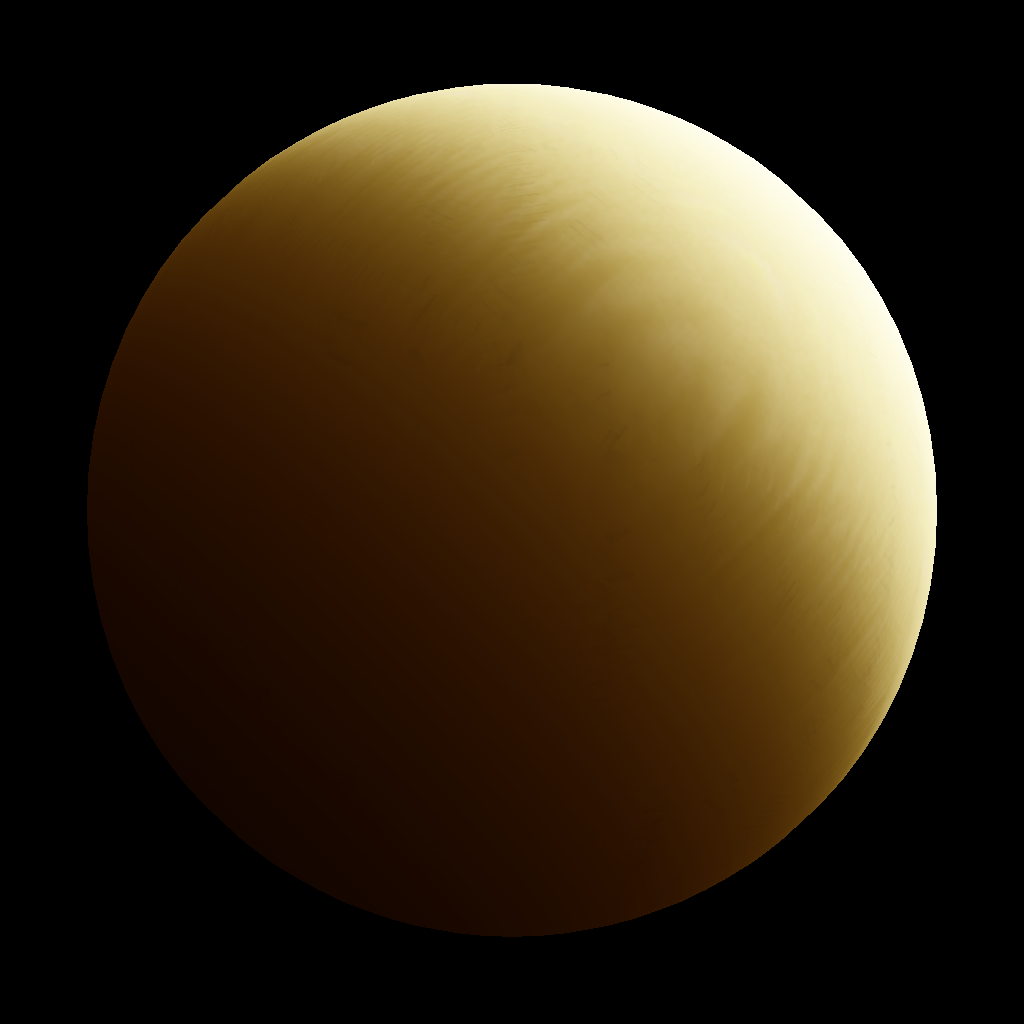
\includegraphics[width=0.25 \textwidth]{p1000}
}
\subfloat[$\ $Reference]{
  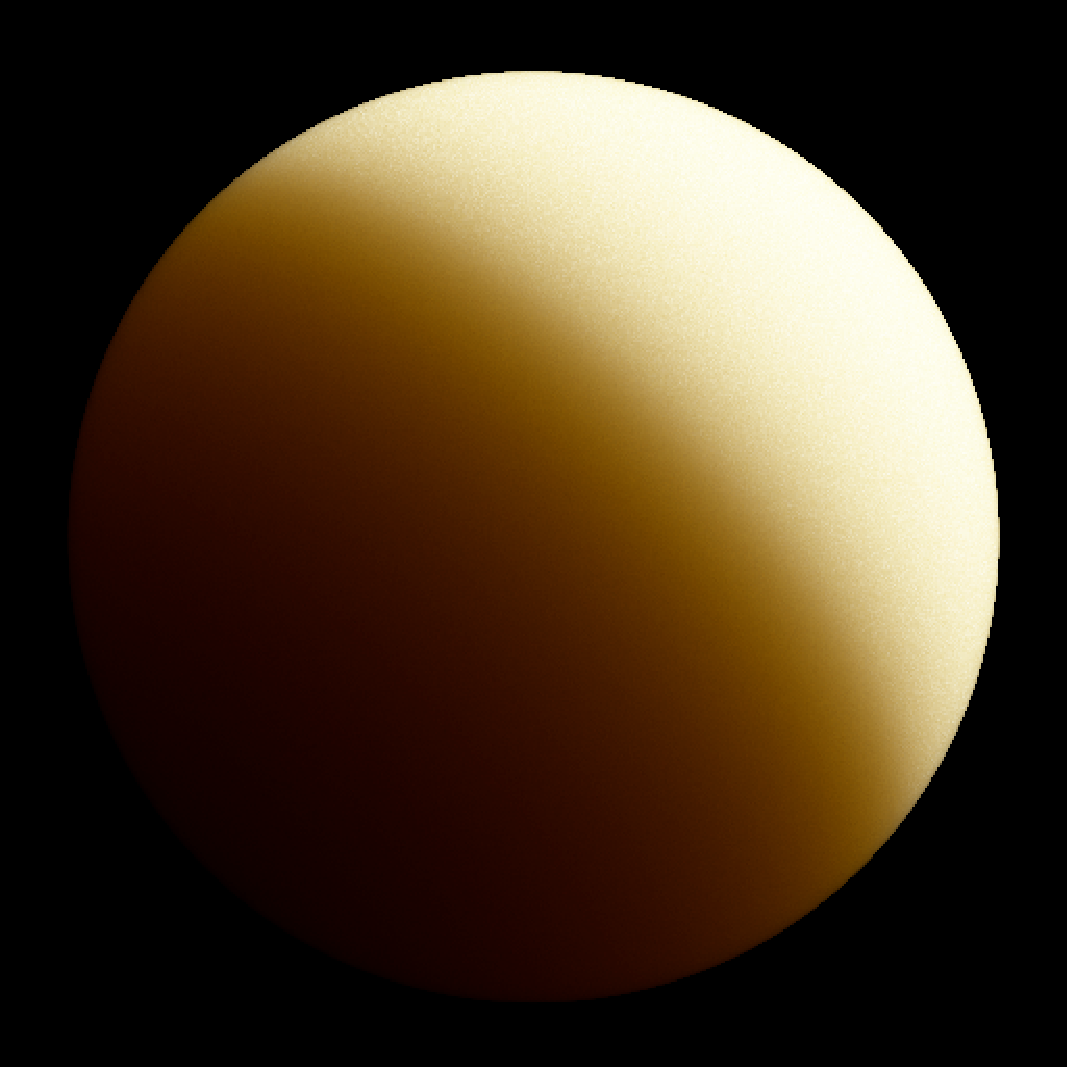
\includegraphics[width=0.25 \textwidth]{p}
} \\
\vspace{-0.4cm}
\subfloat[{$\ N = 100$}]{
  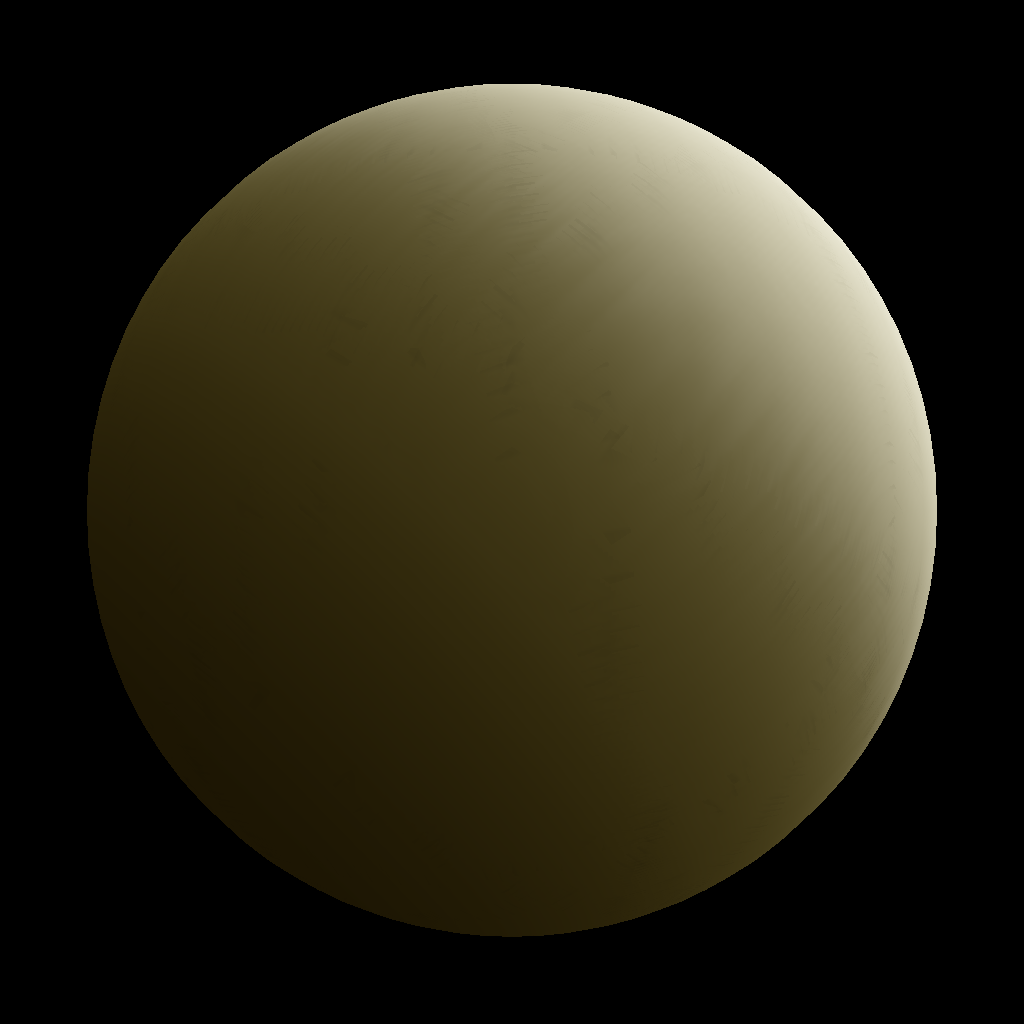
\includegraphics[width=0.25 \textwidth]{gj100}
} 
\subfloat[{$\ N = 1000$}]{
  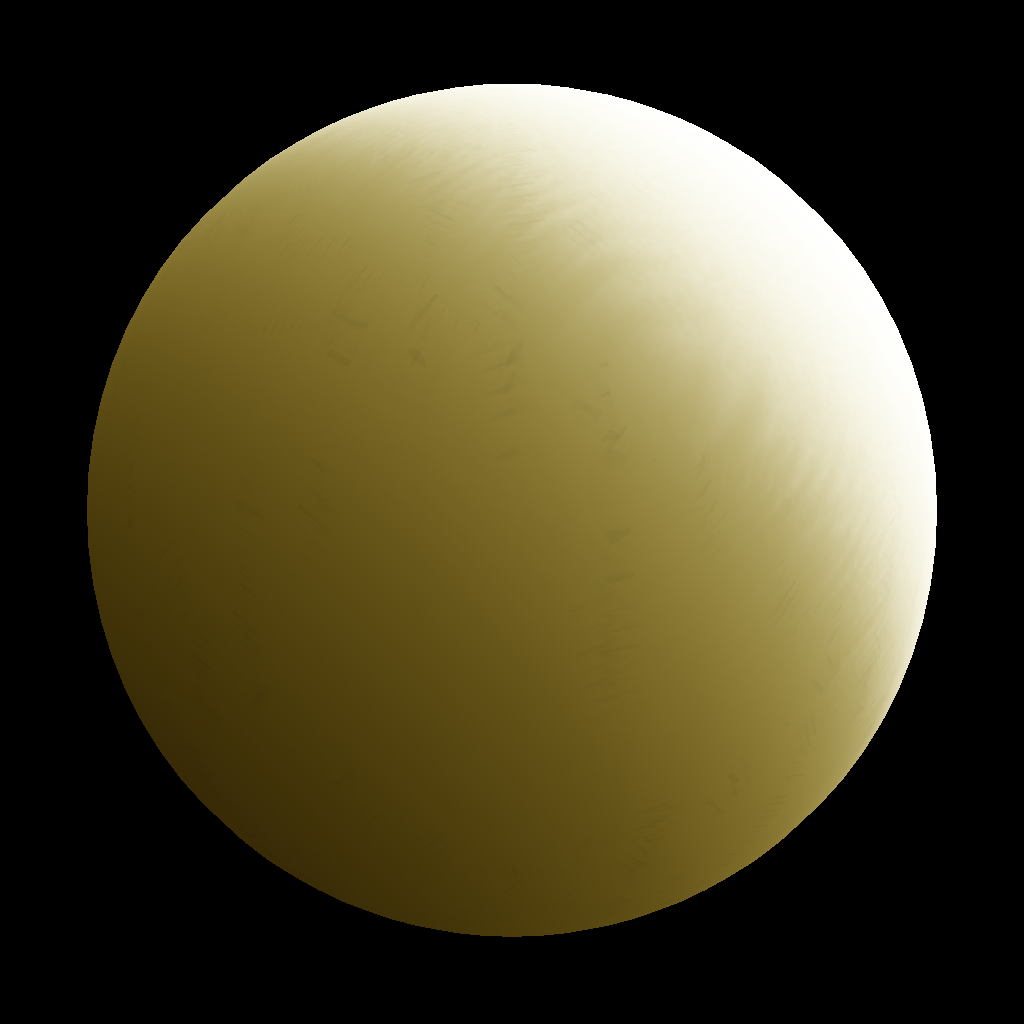
\includegraphics[width=0.25 \textwidth]{gj1000}
} 
\subfloat[$\ $Reference]{
  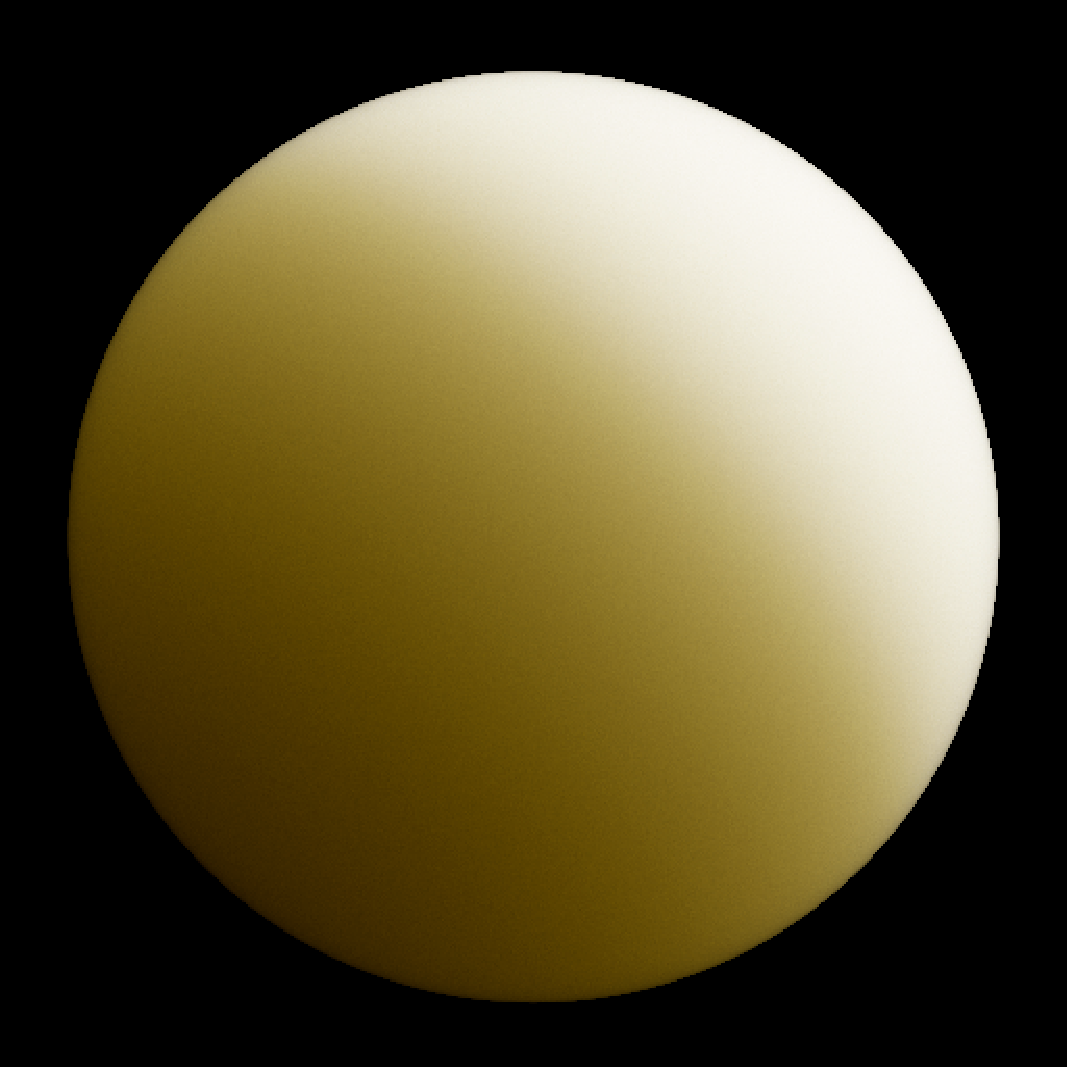
\includegraphics[width=0.25 \textwidth]{gj}
} 
\vspace{-0.2cm}
\caption{Comparison on spheres of potato and white grapefruit juice.}
\end{figure}
\end{frame}



\begin{frame}
    \frametitle{Results (quality)}
				\begin{figure}
\centering
\subfloat[{$\ N = 50$ (ca. 90 milliseconds)}]{
  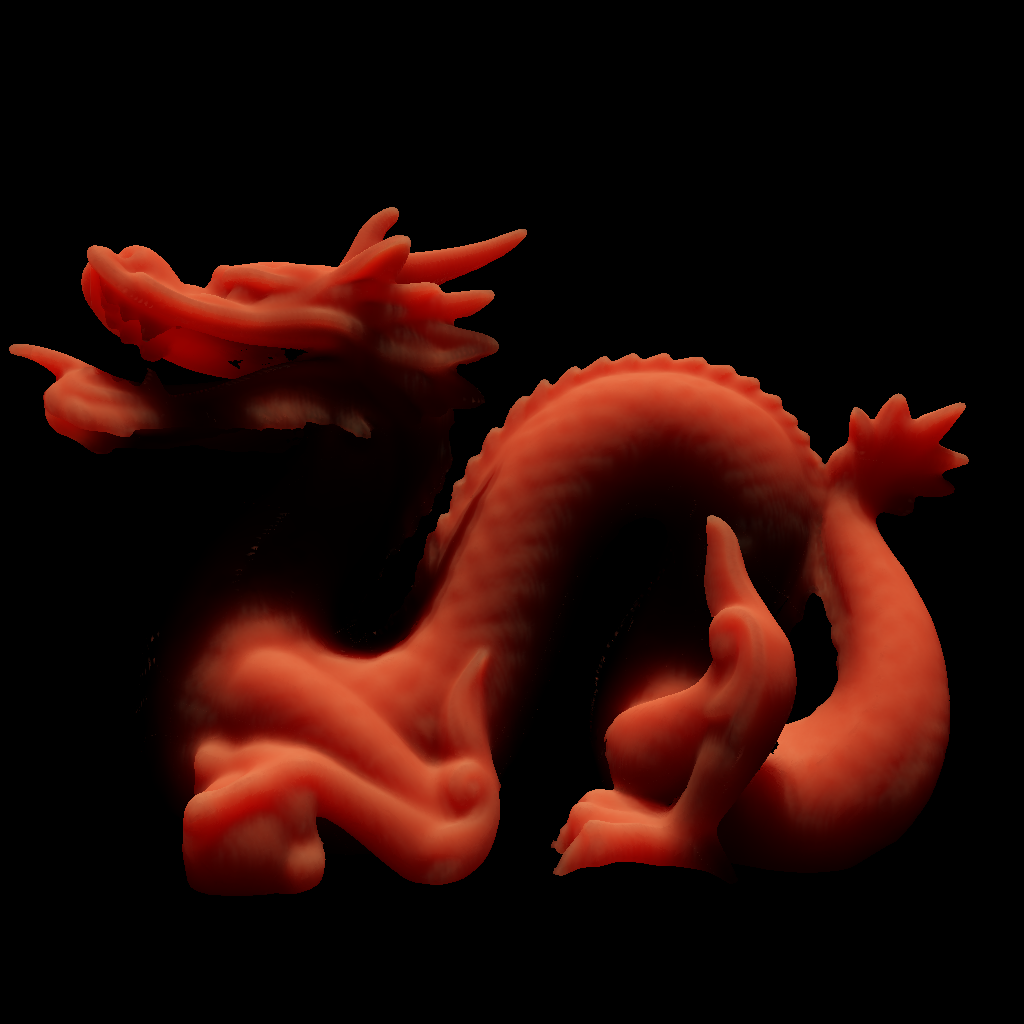
\includegraphics[width=0.45 \textwidth]{d50}
}
\subfloat[$\ $Reference (6 hours, 16 millions samples)]{
  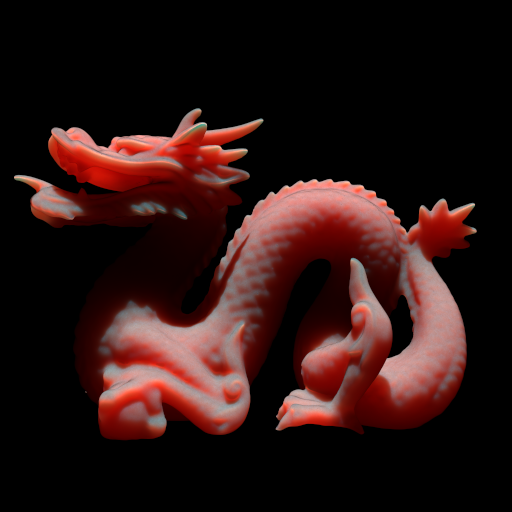
\includegraphics[width=0.45 \textwidth]{d}
} 
\vspace{-0.2cm}
\caption{Result comparison for the Stanford Dragon model. Parameters for ketchup.}
\end{figure}
\end{frame}

\begin{frame}
    \frametitle{Results (quality)}
				\begin{figure}
\centering
\subfloat[{$\ N = 100$}]{
  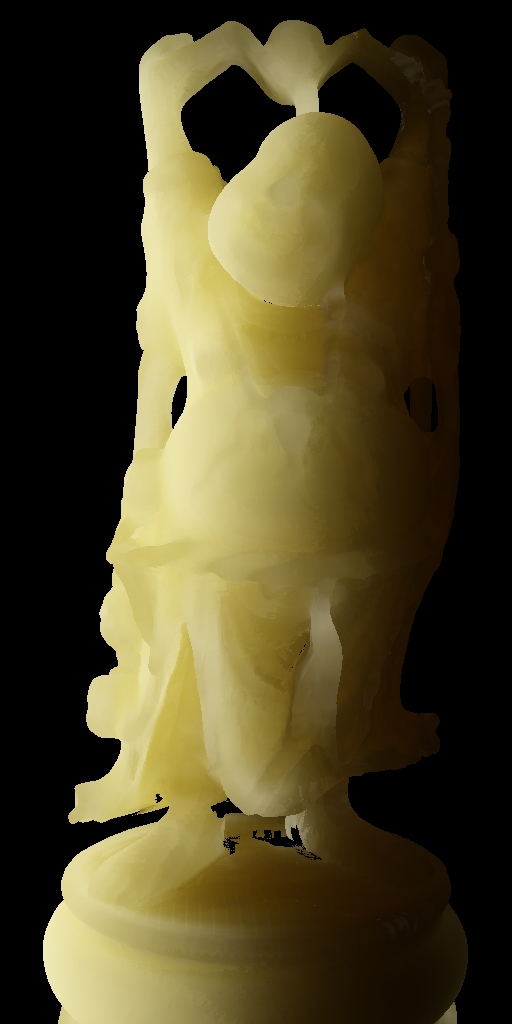
\includegraphics[width=0.25 \textwidth]{b100}
}
\subfloat[$\ $Reference (30 minutes, $10^6$ samples)]{
\makebox[.5\textwidth]{  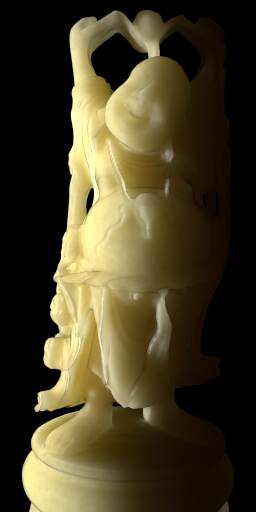
\includegraphics[width=0.25 \textwidth]{bref}
}
} 
\vspace{-0.1cm}
\caption{Result comparison for the Happy Buddha model. Parameters for potato.}
\end{figure}
\end{frame}

\begin{frame}
    \frametitle{Results (quality)}
				\begin{figure}
\centering
\subfloat[{$\ N = 90$}]{
  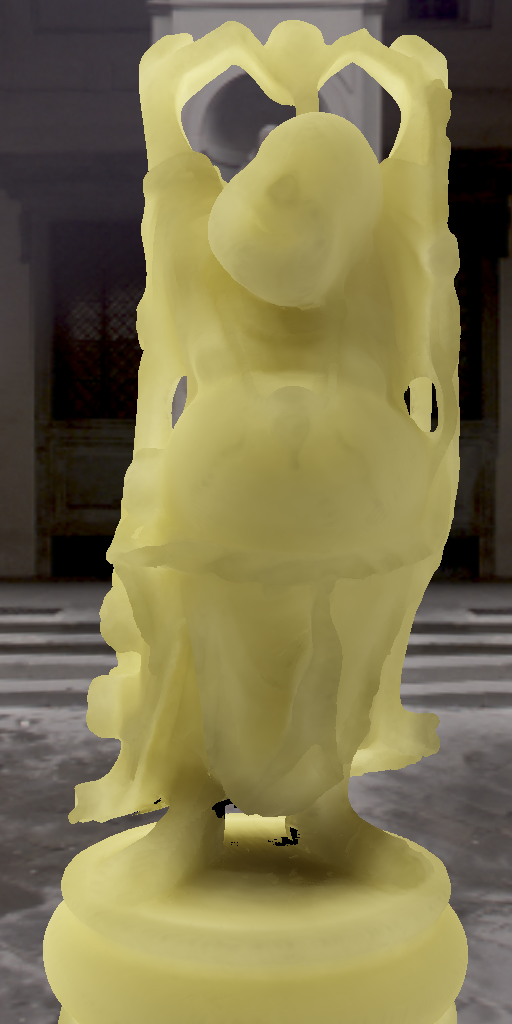
\includegraphics[width=0.25 \textwidth]{env90}
}
\subfloat[$\ $Reference \citep{IMM2013-06646}]{
\makebox[.5\textwidth]{  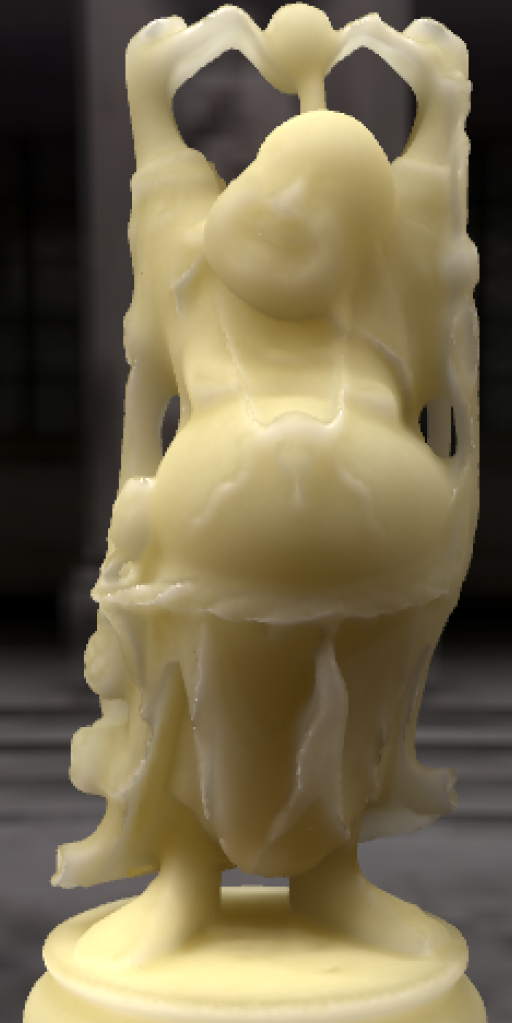
\includegraphics[width=0.25 \textwidth]{envref}
}
} 
\vspace{-0.1cm}
\caption{Result comparison for the Happy Buddha model (environment lighting, Uffizi map). Parameters for potato.}
\end{figure}
\end{frame}

\begin{frame}
    \frametitle{Results (performance)}
		\begin{figure}
\centering
\subfloat[Beer Bunny, $67.7 ms$. Point light. $N = 180$, $M = 210$, $q = 2$]{
  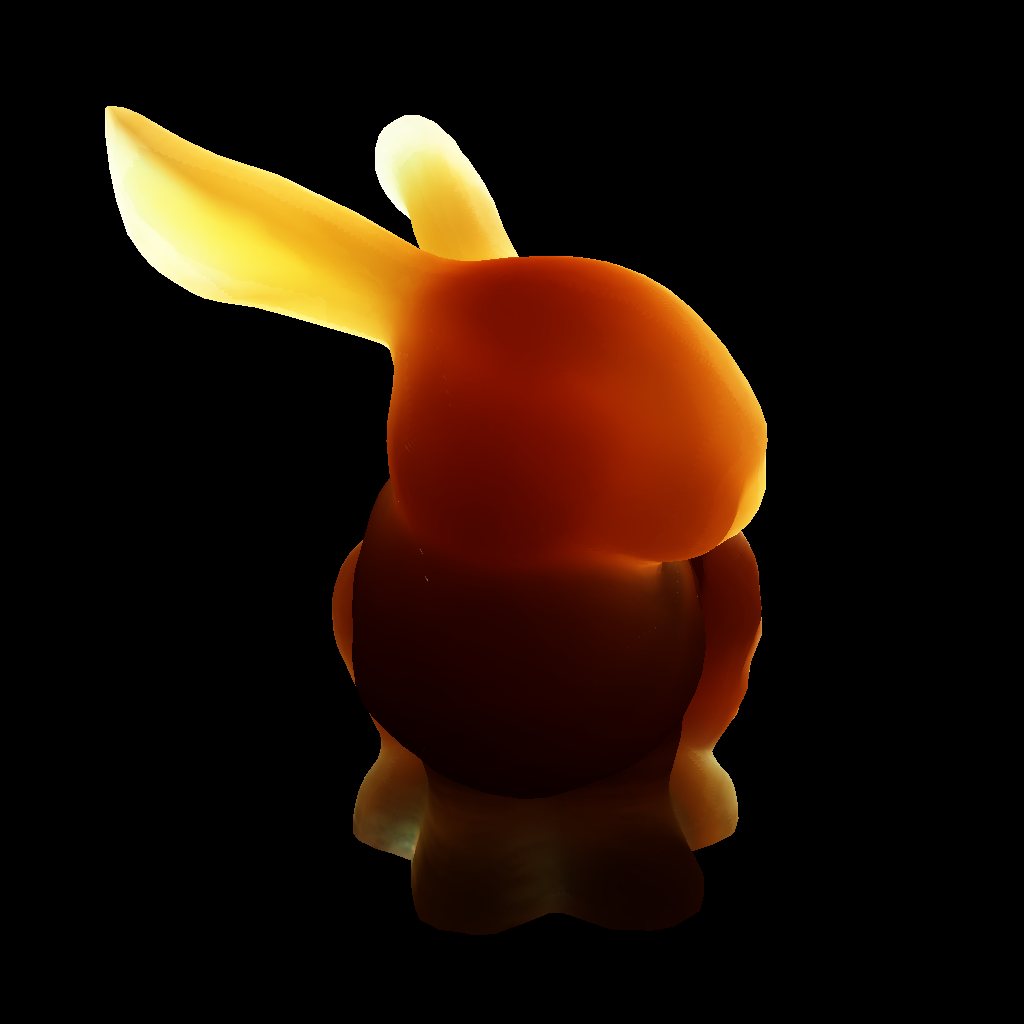
\includegraphics[width=0.4 \linewidth]{example2.png}
}
\subfloat[Detailed timings.]{
\begin{tabular}[b]{lllll}
\multicolumn{5}{c}{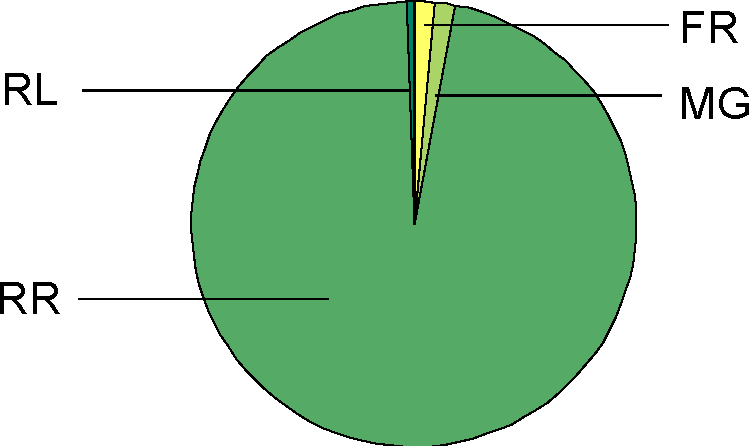
\includegraphics[width=0.3 \linewidth]{bunnychart.pdf}}                                                   \\ \hline
\multicolumn{1}{|l|}{RL}   & \multicolumn{1}{l|}{RR}    & \multicolumn{1}{l|}{MG}   & \multicolumn{1}{l|}{FR}   & \multicolumn{1}{l|}{Tot}   \\ \hline
\multicolumn{1}{|l|}{0.20} & \multicolumn{1}{l|}{66.18} & \multicolumn{1}{l|}{0.8} & \multicolumn{1}{l|}{0.44} & \multicolumn{1}{l|}{67.72} \\ \hline
\end{tabular}
}
\caption{Graph that illustrates how the timings are split into the different phases of the algorithm. All tests use $W_l = W_s = 512$. }
\label{fig:timingssplit}
\end{figure}

\end{frame}


\begin{frame}
    \frametitle{Results (performance)}
\renewcommand{\arraystretch}{1.8}
\begin{table}[!ht]
\centering
\begin{tabular}{p{3cm}l|l|l|l|l|}
\cline{3-6}
                             &      & \multicolumn{4}{c|}{Number of samples ($N$)}                                          \\ \cline{3-6} 
Model                        & \#$\Delta$& \multicolumn{1}{c|}{1} & \multicolumn{1}{c|}{10} & \multicolumn{1}{c|}{50} & \multicolumn{1}{c|}{100} \\ \hline
\multicolumn{1}{|l|}{Bunny}  & $10^4$ & \mycolor{2}.1                  & \mycolor{5}.3                 & \mycolor{19}.8                  & \mycolor{38}.2                 \\ \hline
\multicolumn{1}{|l|}{Dragon} & $10^5$ & \mycolor{12}.5                 & \mycolor{35}.2                  & \mycolor{140}.6                & \mycolor{275}.3                \\ \hline
\multicolumn{1}{|l|}{Buddha} & $10^6$ & \mycolor{96}.7                 & \mycolor{97}.7                  & \mycolor{128}.0                & \mycolor{216}.0                 \\ \hline
\end{tabular}
\caption{Timings in milliseconds of our method for different models and number of samples $N$ (potato material properties). One directional light, 16 directions for rendering and reconstructing.}
\end{table}
\end{frame}

\begin{frame}
    \frametitle{Results (performance)}
		\renewcommand{\arraystretch}{1.8}
\begin{table}[!ht]
\centering
\begin{tabular}{p{3cm}l|l|l|l|l|}

\cline{3-5}
                             &      & \multicolumn{3}{c|}{Size of the radiance map ($W_s$)}                                          \\ \cline{3-5} 
Model                        & \#$\Delta$& \multicolumn{1}{p{1.2cm}|}{256} & \multicolumn{1}{p{1.2cm}|}{512} & \multicolumn{1}{p{1.2cm}|}{1024} \\ \hline
\multicolumn{1}{|l|}{Bunny}  & $10^4$ & \mycolor{11}.4                  & \mycolor{20}.0                 & \mycolor{39}.0                               \\ \hline
\multicolumn{1}{|l|}{Dragon} & $10^5$ & \mycolor{75}.4                 & \mycolor{142}.1                  & \mycolor{299}.4                             \\ \hline
\multicolumn{1}{|l|}{Buddha} & $10^6$ & \mycolor{98}.2                 & \mycolor{127}.0                  & \mycolor{258}.2                             \\ \hline
\end{tabular}
\caption{Timings in milliseconds of our method for different models and size of the radiance map $W_s$ (ketchup material properties). The other parameters were $N = 50$, $L = 1$, $W_l = 512$, $M = 1000$, $K =16$.}
\end{table}
\end{frame}


\begin{frame}
    \frametitle{Results (performance)}
\renewcommand{\arraystretch}{1.8}

\begin{table}[!ht]
\centering
\begin{tabular}{p{3cm}l|l|l|l|l|}
\cline{3-6}
                             &      & \multicolumn{4}{c|}{Number of directions ($K$)}                                          \\ \cline{3-6} 
Model                        & \#$\Delta$& \multicolumn{1}{c|}{4} & \multicolumn{1}{c|}{8} & \multicolumn{1}{c|}{16} & \multicolumn{1}{c|}{32} \\ \hline
\multicolumn{1}{|l|}{Bunny}  & $10^4$ & \mycolor{6}.6                  & \mycolor{10}.0                 & \mycolor{20}.1                  & \mycolor{42}.1                 \\ \hline
\multicolumn{1}{|l|}{Dragon} & $10^5$ & \mycolor{36}.7                 & \mycolor{70}.1                  & \mycolor{143}.0                & \mycolor{306}.2               \\ \hline
\multicolumn{1}{|l|}{Buddha} & $10^6$ & \mycolor{32}.5                 & \mycolor{55}.8                  & \mycolor{128}.3                & \mycolor{363}.5                 \\ \hline
\end{tabular}
\caption{Timings in milliseconds of our method for different models and different number of directions $K$ (ketchup material properties). The other parameters were $N = 50$, $L = 1$, $W_s = W_l = 512$, $M = 1000$.}
\end{table}

\end{frame}


\section{Conclusions}
\begin{frame}
    \frametitle{Conclusions}

\begin{itemize}
\item We implemented a solution for fast rendering of translucent materials using a state of the art directional BSSRDF
\item We obtained results comparable to offline rendered solutions
\item We obtained an improvement of five orders of magnitude over offline rendered solutions
\item We obtained a flexible method that is applicable to current real-time graphics engines
\end{itemize}

\end{frame}

\begin{frame}
    \frametitle{Conclusions}
\centering
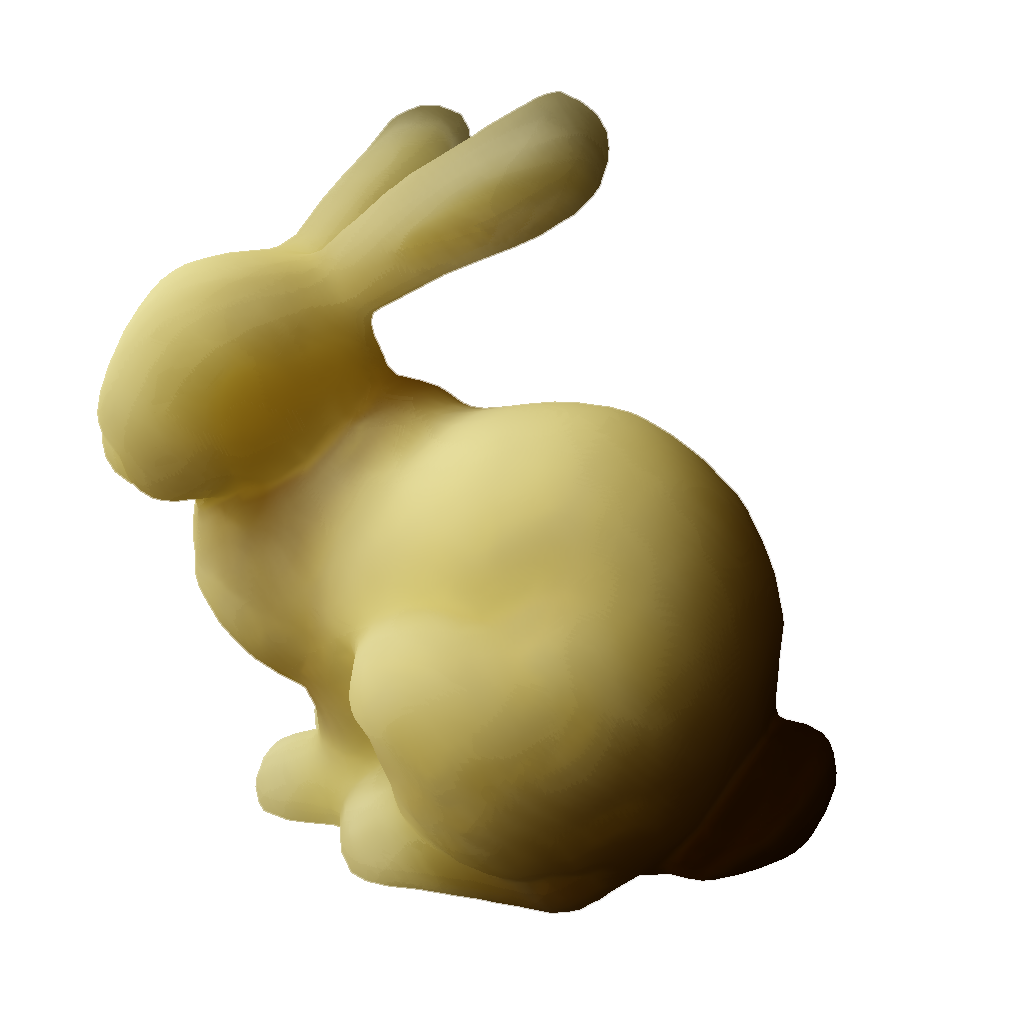
\includegraphics[width=0.4\textwidth]{front} \\
\huge Thank you!
\end{frame}

\section{References}

\begin{frame}
    \frametitle{References}
\bibliographystyle{alexnat}                           %Use alpha codes for references
\bibliography{thesis} 
\end{frame}


\end{document}
